\documentclass[11pt,a4paper]{article}
\usepackage{fontspec}
\setmainfont{Times New Roman}
\setmonofont[Scale=0.88]{Menlo}
\usepackage[margin=2.3cm]{geometry}
\usepackage{booktabs,multirow,graphicx,caption,amsmath,amssymb,enumitem,xcolor,float,array,url}
\usepackage{pgfplots}
\usepackage{tikz}
\usepgfplotslibrary{groupplots}
\usetikzlibrary{positioning,arrows.meta,shapes.geometric,fit,backgrounds}
\usepackage[colorlinks=true,linkcolor=blue!50!black,citecolor=blue!50!black,urlcolor=blue!50!black]{hyperref}
\pgfplotsset{compat=1.17}
\captionsetup{font=small,labelfont=bf,skip=4pt}
\setlist{itemsep=1pt,topsep=3pt}
\renewcommand{\arraystretch}{1.08}
\newcommand{\rl}{ROUGE-L}
\newcommand{\dieu}{\textit{Điều}}
\newcommand{\ci}[2]{{\scriptsize[#1,\,#2]}}
\newcommand{\best}[1]{\textbf{#1}}

\title{\textbf{Improving Retrieval-Augmented Question Answering over Vietnamese Legal Documents\\with a Sub-4B Language Model}\\[2pt]
\large Corpus-aware retrieval, supervised and preference fine-tuning, and a deployable inference stack}
\author{Nguyễn Đắc Hoàng Phú (Student ID: 2670352)\\ Supervisor: Quản Thành Thơ\\ Ho Chi Minh City University of Technology (HCMUT)\\ Large Language Models course --- RAG assignment}
\date{November 2026}

\begin{document}
\maketitle

\begin{abstract}
We study retrieval-augmented question answering (RAG) over Vietnamese legal texts under two constraints: the answering model must have fewer than four billion parameters, and the reference answers follow a rigid template (``\textit{Căn cứ tại khoản $k$ Điều $n$ \ldots\ quy định \ldots}'') followed by a near-verbatim quotation of the cited article. Starting from the course baseline (recursive chunking, a Vietnamese SBERT embedder, FAISS and Qwen1.5-1.8B; test \rl{} $0.171$), we improve each stage of the pipeline and accept a change only when a paired bootstrap on a development split supports it. Three steps carry almost all of the gain: (i)~an index that contains the laws the questions cite (test law-hit rate $0.00\!\to\!0.62$); (ii)~supervised fine-tuning of Qwen3.5-2B on decontaminated pairs with few-shot demonstrations and refusal rows; and (iii)~two rounds of on-policy preference optimisation (DPO) on the model's own best-versus-worst samples. After step~(iii), a single greedy generation matches $8$-sample minimum-Bayes-risk (MBR) decoding. On the held-out test split ($200$ questions) the system reaches \rl{} $0.643$ with one generation per question (cosine $0.916$, token overlap $0.734$, BLEU-1 $0.582$), and $0.652$ with MBR-8. A configuration fixed in advance and retrained on train plus development data lands at $0.640$/$0.646$, inside the seed spread. The same recipe on 4B and 9B models, which exceed the size limit and serve as analysis only, reaches $0.666$ and $0.677$, so model size is a small lever. We also report what did not help (retrieval fine-tuning, legal-domain base models, continued pre-training, agents, thinking-mode training, quantisation), locate the remaining error with oracle analyses, and package the system as a container with three inference endpoints. On one L40S, sequential requests take $2.6$\,s at the median and $6.6$\,s at the p95; two cards serve $15$--$18$ concurrent users within a $10$\,s p95.
\end{abstract}

%------------------------------------------------------------------------------
\section{Introduction}
Retrieval-augmented generation \cite{lewis2020rag,rag_survey} grounds a language model in retrieved passages. Legal question answering is a demanding setting for it:
\begin{itemize}[leftmargin=*]
\item the corpus is large and heavily cross-referenced;
\item answers must cite the right article;
\item a small model that fits on one GPU must reproduce the register of statutory text.
\end{itemize}
The assignment fixes the evaluation (five lexical and semantic similarity metrics against reference answers), limits the answering model to under $4$B parameters, and provides a deliberately naive baseline.

We treat the task as an empirical systems problem. We split the pipeline into retrieval, generation, decoding and post-training, run controlled ablations in each stage, and keep only changes that pass a significance test on a development split. The final system was then checked twice more: by re-running its post-training from other seeds, and by a configuration fixed in advance and scored on test once.

\paragraph{Contributions.}
\begin{enumerate}[leftmargin=*]
\item \textbf{Corpus-aware retrieval.} One chunk per \dieu, cleaning and de-duplication, an index extended with the laws the QA set cites, then dense top-50 and a cross-encoder reranker. The share of questions whose cited law can be retrieved rises from $0$ to $0.62$. With an untuned Vietnamese 3B generator, test \rl{} rises from $0.171$ to $0.443$ (Section~\ref{sec:retrieval}).
\item \textbf{A supervised recipe for a 2.27B model}: decontaminated pairs, few-shot demonstrations drawn from the nearest training questions, gold-passage injection and refusal rows. Fine-tuning is worth $+0.23$ dev \rl{} over the raw model. The recipe adds $+0.03$ over plain fine-tuning on dev, mostly through the two demonstrations at inference, and does not carry over to test ($-0.010$, n.s.; Section~\ref{sec:generator}).
\item \textbf{On-policy, iterated DPO} on best-versus-worst self-samples, scored by the evaluation metric itself:
  \begin{itemize}[leftmargin=*]
  \item two rounds add $+0.031$ dev \rl{} \ci{+0.014}{+0.049} over the supervised model under greedy decoding, of which round~2 alone contributes $+0.009$ (n.s.);
  \item a third round degrades the model;
  \item across seeds, the first round is robust, but the second round's extra gain is not always reproduced (Section~\ref{sec:posttrain}).
  \end{itemize}
\item \textbf{A record of what did not help}, with an oracle analysis showing that the remaining error lies in which clause is quoted and how much of it, not in retrieval (Sections~\ref{sec:analysis} and~\ref{sec:negative}). A scaling check with the same recipe on 4B and 9B models adds only $+0.023$ and $+0.034$ test \rl{} (Section~\ref{sec:scaling}).
\item \textbf{A containerised QA service} with separate LLM, embedding and reranking endpoints and a refusal guard for off-topic questions, with measured latency, capacity and engine settings (Section~\ref{sec:deploy}).
\end{enumerate}

%------------------------------------------------------------------------------
\section{Related Work}
\paragraph{Retrieval-augmented generation and legal NLP.}
RAG combines a retriever with a generator \cite{lewis2020rag}; \cite{rag_survey} survey chunking, retrieval, reranking and generation choices. Legal NLP has English benchmarks \cite{lexglue,legalbench}. For Vietnamese there are pretrained legal models \cite{vilegallm}, built on Vietnamese encoders \cite{phobert} or on multilingual decoder families \cite{qwen25,qwen3}. Reported Vietnamese legal results mostly concern retrieval or classification. Free-form answers scored against references, the setting studied here, are rarely reported.
\paragraph{Retrieval and reranking.}
Dense bi-encoders \cite{dpr,sbert,bgem3} retrieve candidates cheaply; cross-encoders \cite{monobert} re-score a short list more accurately. Lexical scoring \cite{bm25} can be fused with dense ranks \cite{rrf}. We follow this two-stage design and measure each component. Context length matters for the generator \cite{lostmiddle}, which is a reason to keep the number of passages small.
\paragraph{Adapting small generators.}
Parameter-efficient fine-tuning \cite{lora,pissa} and retrieval-aware training with distractor and injected gold passages \cite{raft} can teach a small model the answer register. Policy-gradient methods \cite{ppo,instructgpt} and their group-relative variants \cite{grpo,r1} optimise a verifiable reward. DPO \cite{dpo} and reference-free relatives \cite{simpo} optimise preferences without a reward model. Weight-space operations \cite{soups,taskarith} combine checkpoints, and rationalisation \cite{star} produces reasoning traces for supervised training. We use the evaluation metric itself as the reward and apply DPO \emph{on-policy and iteratively}.
\paragraph{Decoding and agents.}
Minimum-Bayes-risk decoding \cite{mbr,freitag} and self-consistency \cite{selfcons} choose among samples by agreement. Agentic RAG with tools \cite{react,selfrag,searchr1} lets the model decide what to retrieve. We show that MBR recovers only part of the best-of-$n$ headroom and that DPO can move that selection into the model. With a 2B model and retrieval already near its ceiling, agents did not help.

%------------------------------------------------------------------------------
\section{Task, Data and Evaluation Protocol}\label{sec:data}

\subsection{Corpus}
The course corpus has $16{,}441$ plain-text legal documents ($428$\,MB; $63.1$M words; median $2{,}224$ words per document).
\begin{itemize}[leftmargin=*]
\item \textbf{Issuers:} local regulations dominate (Địa phương $64.8\%$), followed by ministries ($23.3\%$), the Government ($7.3\%$) and the National Assembly ($0.4\%$).
\item \textbf{Types:} decisions (\textit{Quyết định}) are $54.8\%$ of all documents.
\item \textbf{Articles:} $12{,}272$ documents contain at least one \dieu{} ($84{,}222$ articles in total).
\item \textbf{Years:} 1929 to 2025, median 2015.
\item \textbf{Relations:} documents carry relation blocks (``based on'', ``replaced by'', \ldots) that give $190{,}981$ edges.
\end{itemize}

\subsection{Question--answer set and splits}
The QA set has $2{,}745$ question/reference pairs. Questions have a median of $137$ characters; references a median of $1{,}426$ and a maximum of $9{,}858$. References follow a template and quote the cited article almost verbatim, so lexical metrics reward citing and quoting the right article. A fixed seeded split gives $2{,}245$ training, $300$ development and $200$ test pairs.

\paragraph{Corpus--question mismatch.}
The questions mostly cite laws that the course corpus does not contain:
\begin{itemize}[leftmargin=*]
\item only $8$ law identifiers ($51$ QA rows) match a file of the course corpus;
\item $772$ rows have no extractable law identifier;
\item the most frequently cited laws are 2024--2025 banking circulars absent from the corpus.
\end{itemize}
As a result, the baseline retrieves the cited law for essentially no question (law-hit $0$). We therefore extend the retrieval store with:
\begin{enumerate}[leftmargin=*,label=(\roman*)]
\item central-government documents from a public Vietnamese legal-document dataset (first those issued since 2010, selected by a metadata rule fixed before looking at the questions; the final store widens this to 2000);
\item every document that a QA answer cites and that is missing from both sources, crawled from a public legal portal.
\end{enumerate}
After exact and near-duplicate removal ($186$ documents dropped), the final store holds $46{,}498$ documents ($724{,}215$ chunks). Appendix~\ref{app:data} lists further data checks.

\paragraph{Decontamination.}
Nothing a model is trained on may contain knowledge tied to the test split. We drop training and development pairs that either:
\begin{itemize}[leftmargin=*]
\item cite the same (law, \dieu) as a test answer ($16\%$ of train), or
\item share a non-boilerplate 13-gram with a test answer ($20\%$ of train).
\end{itemize}
After filtering, $1{,}452$ training and $188$ development pairs remain for fine-tuning. The retrieval store may contain full laws but never test question/answer pairs.

\paragraph{Development subsets.}
Dev overlaps more with the retained training pairs than test does:
\begin{itemize}[leftmargin=*]
\item $45\%$ of development questions share a \dieu{} with retained training pairs (test: $0\%$);
\item $72\%$ share a 13-gram (test: $32\%$).
\end{itemize}
Plain dev is therefore optimistic for fine-tuned models, and we report three views:
\begin{itemize}[leftmargin=*]
\item \texttt{dev} ($300$ questions);
\item \texttt{dev\_clean} ($166$; no shared \dieu);
\item \texttt{dev\_strict} ($74$; additionally no shared non-boilerplate 13-gram), the closest to the test condition.
\end{itemize}

\subsection{Metrics and significance}
We report the five course metrics, computed with a line-for-line port of the baseline code on lower-cased, punctuation-stripped text:
\begin{itemize}[leftmargin=*]
\item cosine similarity of Vietnamese SBERT embeddings;
\item Jaccard;
\item token overlap;
\item unigram BLEU with brevity penalty;
\item \rl{} F1 \cite{rouge}, the primary metric.
\end{itemize}
Differences between systems are assessed with a paired bootstrap over questions \cite{bootstrap,bergk} ($95\%$ intervals). A change is \emph{accepted} only if the lower bound of its interval is positive on \texttt{dev} and the difference is not negative on \texttt{dev\_clean} or \texttt{dev\_strict}. Run-to-run noise is not negligible: identical vLLM runs differ by about $\pm0.003$ \rl{} with greedy decoding and by about $\pm0.006$ with $8$-sample MBR.

\paragraph{Use of the test split.}
Model and hyper-parameter selection used the development split. The test split was scored at four points, and each is reported:
\begin{enumerate}[leftmargin=*]
\item for configurations of the main development line, as a progress check that was not used for selection (Appendix~\ref{app:test});
\item for the later PiSSA-based recipes, which were compared on dev \emph{and} test, so test is not untouched for those comparisons (Section~\ref{sec:pissa});
\item once for a configuration fixed in advance (Section~\ref{sec:finalchain});
\item once per decoding mode for the 4B and 9B scaling points, after all their training was done; they are analysis only and could not be selected (Section~\ref{sec:scaling}).
\end{enumerate}
The retrieval tables (Tables~\ref{tab:corpus}, \ref{tab:retrabl} and~\ref{tab:chunk}) also show test-split retrieval numbers next to dev; every retrieval choice was made on dev.

%------------------------------------------------------------------------------
\section{Method}\label{sec:method}
\begin{figure}[t]
\centering
\resizebox{\linewidth}{!}{%
\begin{tikzpicture}[node distance=6mm and 4mm, every node/.style={font=\footnotesize},
 box/.style={draw,rounded corners=2pt,minimum height=8mm,align=center,fill=blue!6},
 model/.style={draw,rounded corners=2pt,minimum height=8mm,align=center,fill=orange!12},
 arr/.style={-{Stealth[length=2mm]},thick}]
 \node[box] (q) {Question};
 \node[model,right=of q] (emb) {Embedder\\{\scriptsize endpoint}};
 \node[box,right=of emb] (faiss) {FAISS dense\\top-50};
 \node[model,right=of faiss] (rr) {Reranker\\{\scriptsize endpoint}};
 \node[box,right=of rr] (top) {top-5 \dieu};
 \node[box,fill=gray!15,below=9mm of top] (guard) {Refusal guard\\(best rerank score $\geq\tau$)};
 \node[box,left=of guard] (prompt) {Prompt:\\2 shots + 5 \dieu\ + question};
 \node[model,left=of prompt] (llm) {LLM (DPO)\\{\scriptsize endpoint, greedy}};
 \node[box,left=of llm] (ans) {Answer\\+ sources};
 \draw[arr] (q)--(emb); \draw[arr] (emb)--(faiss); \draw[arr] (faiss)--(rr); \draw[arr] (rr)--(top);
 \draw[arr] (top)--(guard); \draw[arr] (guard)--(prompt); \draw[arr] (prompt)--(llm); \draw[arr] (llm)--(ans);
 \draw[arr,dashed] (guard.south) -- ++(0,-5mm) -| node[pos=0.25,below]{score $<\tau$: fixed refusal, no LLM call} (ans.south);
\end{tikzpicture}}
\caption{The deployed pipeline. Embedder, reranker and LLM are independent inference endpoints; the QA service holds only the index and the few-shot pool.}\label{fig:pipeline}
\end{figure}

\subsection{Retrieval}
\begin{enumerate}[leftmargin=*]
\item \textbf{Preparation.} Documents are cleaned (headers, signatures and tails removed), de-duplicated, and split into one chunk per \dieu. Long articles are split at $2{,}000$ characters with an overlap of $100$.
\item \textbf{Dense retrieval.} Chunks are embedded with the AITeamVN Vietnamese Embedding model (568M parameters, $512$ tokens; a bge-m3-style encoder \cite{bgem3} fine-tuned for Vietnamese) into an inner-product FAISS index \cite{faiss}, which returns the top $50$.
\item \textbf{Reranking.} The AITeamVN Vietnamese Reranker cross-encoder \cite{monobert} (max length $1{,}024$) re-scores these $50$, and the top $k{=}5$ go to the generator.
\end{enumerate}
Both encoder models are served by vLLM \cite{vllm} pooling servers. The pipeline is built with LlamaIndex \cite{llamaindex}; training uses TRL \cite{trl}.

\subsection{Generator and supervised fine-tuning}
The answering model is Qwen3.5-2B ($2.27$B parameters; we write ``2B'' for short; Qwen family \cite{qwen3}) with thinking mode disabled. The prompt contains:
\begin{itemize}[leftmargin=*]
\item the retrieved \dieu{} passages;
\item optionally two demonstrations: the nearest decontaminated training questions by token Jaccard, with their reference answers;
\item the question.
\end{itemize}
Supervised fine-tuning uses LoRA \cite{lora} ($r{=}32$, all linear layers) on the decontaminated pairs, rendered with exactly the inference prompt; the loss covers the answer only. The final recipe, \emph{v3b}, combines four elements:
\begin{enumerate}[leftmargin=*,label=(\alph*)]
\item a random number $k\in[3,10]$ of passages per example;
\item \emph{gold injection}: when retrieval missed the gold \dieu, it is inserted with probability $0.7$ (RAFT-style \cite{raft});
\item $0$--$3$ demonstrations per example;
\item with probability $0.2$, an extra row whose context was retrieved for an unrelated question and whose target is a refusal.
\end{enumerate}
Training runs $3$ epochs (effective batch $16$, max length $12{,}288$). A later variant initialises the adapter from the principal singular vectors of the weights (PiSSA \cite{pissa}); Section~\ref{sec:pissa} reports it.

\subsection{Decoding}
\textbf{Greedy} decoding (temperature $0$, top-$p$ $0.95$, $\le 1{,}024$ new tokens) needs one generation per question.

\textbf{MBR} decoding \cite{mbr} samples $n{-}1$ candidates at temperature $0.7$ in addition to the greedy one. It returns the candidate with the highest mean \rl{} to the others:
\begin{equation}
\hat y=\arg\max_{y\in\mathcal C}\sum_{y'\in\mathcal C\setminus\{y\}}\operatorname{ROUGE\text{-}L}(y,y').
\end{equation}
MBR trades $n\times$ generation cost for consensus quality.

\subsection{Post-training with the evaluation metric as reward}
\paragraph{Reward.} Both post-training methods score an answer against the reference with
\begin{equation}
R=0.6\,\mathrm{RL}+0.2\,\mathrm{TO}+0.2\,\mathrm{cite}-p_{\mathrm{copy}}-p_{\mathrm{len}},
\end{equation}
where:
\begin{itemize}[leftmargin=*]
\item $\mathrm{RL}$ is \rl{} and $\mathrm{TO}$ is token overlap;
\item $\mathrm{cite}$ is the fraction of the reference's \dieu{} numbers that appear in the answer;
\item $p_{\mathrm{copy}}$ penalises copying more than $90\%$ of the prompt's 8-grams;
\item $p_{\mathrm{len}}$ is a two-sided band around the reference length.
\end{itemize}
A cosine variant replaces part of the lexical weight by sentence-embedding cosine.

\paragraph{GRPO.} Group-Relative Policy Optimisation \cite{grpo} uses $8$ completions per prompt, LoRA $r{=}32$, and no KL term unless stated.

\paragraph{On-policy DPO.}
\begin{enumerate}[leftmargin=*]
\item For each training prompt, draw $8$ samples from the current model: the greedy one and $7$ at $T{=}0.7$.
\item Score them with the reward above.
\item Form one preference pair (best, worst) when the reward gap is $\ge0.1$ and the reference is not a refusal.
\item Train Direct Preference Optimisation \cite{dpo} on these pairs: LoRA $r{=}32$, $\beta{=}0.1$, learning rate $2\!\times\!10^{-5}$, one epoch, effective batch $16$; the reference model is the policy with its adapter disabled.
\end{enumerate}
\emph{Iterating}, i.e.\ sampling again from the improved model, gives round~2.

\paragraph{Weight-space merging.} We also test weight averaging \cite{soups} and task arithmetic \cite{taskarith}, $\theta=\theta_{\mathrm{SFT}}+\alpha(\theta_{\mathrm{RL}}-\theta_{\mathrm{base}})$.

%------------------------------------------------------------------------------
\section{Results}\label{sec:results}

\subsection{Main results on the test split}
Table~\ref{tab:main} follows the system from the course baseline to the final model, and Figure~\ref{fig:ladder} plots the same path.
\begin{table}[H]
\centering
\caption{Test split ($n{=}200$, no errors). The first row is the course baseline (answer-only decoding). The final system is SFT v3b followed by two DPO rounds.}\label{tab:main}
\begin{tabular}{@{}lccccc@{}}
\toprule
System & Cos. & Jacc. & Tok. & BLEU-1 & \rl{}\\
\midrule
Course baseline (SBERT + Qwen1.5-1.8B) & .602 & .164 & .191 & .138 & .171\\
+ better embedder/reranker, Vi-Qwen2-3B-RAG & .671 & .226 & .211 & .126 & .171\\
+ index with cited laws (A2e) & .812 & .500 & .555 & .412 & .443\\
SFT Qwen3.5-2B (v0), greedy & .905 & .658 & .754 & .563 & .618\\
SFT v0 + MBR-8 & .915 & .677 & .761 & .599 & .645\\
SFT v3b (2 shots), greedy & .905 & .656 & .735 & .538 & .607\\
\midrule
\best{Final: SFT v3b + 2 DPO rounds, greedy} & \best{.916} & \best{.673} & \best{.734} & \best{.582} & \best{.643}\\
Final + MBR-8 & .918 & .681 & .728 & .587 & \best{.652}\\
Final, second DPO seed, greedy & .915 & .665 & .707 & .578 & .638\\
\bottomrule
\end{tabular}
\end{table}

\begin{figure}[H]
\centering
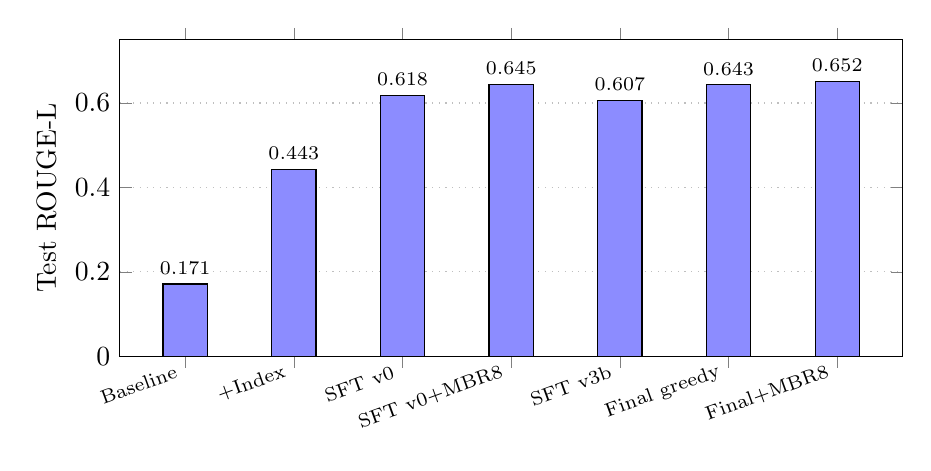
\begin{tikzpicture}
\begin{axis}[ybar,width=0.95\linewidth,height=5.6cm,bar width=16pt,ymin=0,ymax=0.75,
 symbolic x coords={Baseline,+Index,SFT v0,SFT v0+MBR8,SFT v3b,Final greedy,Final+MBR8},xtick=data,
 x tick label style={font=\scriptsize,rotate=20,anchor=east},ylabel={Test \rl{}},
 nodes near coords,nodes near coords style={font=\scriptsize},every node near coord/.append style={/pgf/number format/fixed,/pgf/number format/precision=3},
 ymajorgrids,grid style={dotted}]
\addplot[fill=blue!45] coordinates {(Baseline,0.171)(+Index,0.443)(SFT v0,0.618)(SFT v0+MBR8,0.645)(SFT v3b,0.607)(Final greedy,0.643)(Final+MBR8,0.652)};
\end{axis}
\end{tikzpicture}
\caption{Test \rl{} along the development of the system. The final system builds on SFT v3b; SFT v0 is the plain fine-tuned model.}\label{fig:ladder}
\end{figure}

\paragraph{Significance on test.}
Table~\ref{tab:testboot} gives paired-bootstrap differences ($10{,}000$ resamples over the $200$ test questions).
\begin{itemize}[leftmargin=*]
\item The improvement over the baseline is large on every metric.
\item The final greedy system is significantly better than both supervised models.
\item Adding MBR-8 on top of the final system, or switching to the second DPO seed, cannot be distinguished from the final greedy system.
\end{itemize}
The single-generation system is therefore the recommended one.
\begin{table}[H]
\centering
\caption{Paired bootstrap on the test split ($n{=}200$): mean difference (B$-$A) with $95\%$ interval.}\label{tab:testboot}
\begin{tabular}{@{}llccc@{}}
\toprule
A & B & Metric & Difference & $95\%$ CI\\
\midrule
Course baseline & Final, greedy & \rl{} & $+.472$ & \ci{+.439}{+.505}\\
 & & BLEU-1 & $+.444$ & \ci{+.407}{+.479}\\
 & & Cosine & $+.314$ & \ci{+.292}{+.336}\\
 & & Jaccard & $+.509$ & \ci{+.478}{+.539}\\
 & & Token overlap & $+.543$ & \ci{+.509}{+.576}\\
SFT v0, greedy & Final, greedy & \rl{} & $+.026$ & \ci{+.004}{+.049}\\
SFT v3b, greedy & Final, greedy & \rl{} & $+.036$ & \ci{+.013}{+.058}\\
SFT v0, greedy & SFT v0, MBR-8 & \rl{} & $+.028$ & \ci{+.011}{+.044}\\
SFT v0, MBR-8 & Final, MBR-8 & \rl{} & $+.007$ & \ci{-.014}{+.028} (n.s.)\\
Final, greedy & Final, MBR-8 & \rl{} & $+.009$ & \ci{-.004}{+.022} (n.s.)\\
Final, seed 2, greedy & Final, greedy & \rl{} & $+.006$ & \ci{-.009}{+.019} (n.s.)\\
\bottomrule
\end{tabular}
\end{table}

\subsection{Retrieval study}\label{sec:retrieval}
\paragraph{Corpus coverage is the dominant factor.}
Table~\ref{tab:corpus} varies the retrieval store with the generator fixed (Vi-Qwen2-3B-RAG, no fine-tuning). Cleaning and per-\dieu{} chunking change nothing (A2a/A2b), because the cited laws are simply absent. Adding central-government laws (A2c, a test-blind rule: issued since 2010) and then every document the QA set cites (A2d, since 2000) raises dev law-hit from $\approx0.02$ to $0.58$--$0.63$ ($0.62$ on test for the final store) and \rl{} from $0.17$ to $0.42$ on dev ($0.44$ on test).
\begin{table}[H]
\centering
\caption{Effect of the retrieval store (dev $n{=}300$; test in parentheses, not used for selection). Law-hit (dev) = fraction of questions whose cited law is among the retrieved passages.}\label{tab:corpus}
\begin{tabular}{@{}llccc@{}}
\toprule
Id & Store & Law-hit & \rl{} dev & \rl{} test\\
\midrule
A2a & course corpus, cleaned, recursive chunks & .013 & .170 & (.176)\\
A2b & course corpus, one chunk per \dieu & .017 & .171 & (.176)\\
A2c & + central-government laws since 2010 & .590 & .415 & (.437)\\
A2d & + all cited laws (portal crawl), $\ge$2000 & .577 & .421 & (.444)\\
A2e & + near-duplicate removal & \best{.633} & \best{.423} & (.443)\\
\bottomrule
\end{tabular}
\end{table}

\paragraph{The two-stage stack.}
Table~\ref{tab:retrabl} compares retrievers on the final store.
\begin{itemize}[leftmargin=*]
\item \textbf{Lexical retrieval is far weaker} than the dense embedder (Doc@5 $.65$ against $.89$). Fusing it with dense results lowers recall compared with dense alone.
\item \textbf{Hybrid after reranking} is on par with dense on dev but not better, so we keep the simpler dense-plus-reranker stack.
\item \textbf{Reranking} adds about $+0.04$ Doc@5 and $+0.06$ \dieu{}@5; at the retrieval level its depth ($20$--$100$ candidates) matters little.
\item \textbf{More passages buy little recall:} on test, \dieu{}@5/10/20 is $.898/.944/.966$. For the fine-tuned generator, $k{=}10$ was worse than $k{=}5$ (dev \rl{} $.612$ against $.633$ for v3b), consistent with long contexts diluting the relevant passage \cite{lostmiddle}.
\end{itemize}
\begin{table}[H]
\centering
\caption{Retrieval variants (retrieval only, top-10 returned; dev / test). Documents $n{=}281/193$ and articles $n{=}264/177$ have a recoverable gold. ``+rr$N$'' = reranker over $N$ candidates; hybrid = reciprocal-rank fusion of dense and BM25. The fine-tuned reranker was trained on $4{,}015$ groups (gold \dieu{} positives, dense hard negatives).}\label{tab:retrabl}
\begin{tabular}{@{}lccccc@{}}
\toprule
Retriever & Doc@1 & Doc@5 & \dieu{}@1 & \dieu{}@5 & Doc MRR\\
\midrule
Dense (no reranker) & .619/.596 & .890/.891 & .542/.548 & .845/.842 & .737/.721\\
Dense + rr20 & .651/.648 & .929/.928 & .591/.610 & .894/.904 & .775/.761\\
\textbf{Dense + rr50 (final)} & .644/.648 & \best{.932}/.922 & .591/.610 & \best{.905}/.898 & .769/.760\\
Dense + rr100 & .644/.648 & .929/.907 & .587/.610 & .898/.887 & .767/.758\\
BM25 & .434/.389 & .648/.648 & .250/.288 & .496/.509 & .525/.488\\
BM25 + rr & .587/.586 & .833/.788 & .515/.542 & .754/.712 & .693/.672\\
Hybrid (RRF) & .541/.539 & .851/.824 & .432/.452 & .761/.751 & .674/.661\\
Hybrid + rr & .637/.643 & .936/.912 & .580/.610 & .905/.893 & .768/.753\\
Dense + fine-tuned rr50 (dev only) & -- & -- & .712 & -- & --\\
\bottomrule
\end{tabular}
\end{table}

\paragraph{Better ranking does not reach the answer.}
Every attempt to improve the ranking itself left generation unchanged:
\begin{itemize}[leftmargin=*]
\item \textbf{Fine-tuned reranker.} Raises pipeline \dieu{}@1 from about $.59$ (Table~\ref{tab:retrabl}) to $.712$ on dev, but generation does not improve ($.6325\to.6253$).
\item \textbf{Fine-tuned embedder.} The best of fifteen variants (LoRA or full, several learning rates) gains $+0.023$ \dieu{}@1 \ci{+0.004}{+0.045}, which does not meet the acceptance rule.
\item \textbf{Other zero-shot embedders.} AITeamVN's embedder (\dieu{}@1 $.534$, MRR $.674$ on its own top-50 pool) beat bge-m3 ($.523$) and Qwen3-Embedding-4B/8B ($.51$, 9--12$\times$ slower).
\item \textbf{Chapter/scope prefixes and a kNN prior.} Embedding the chapter/scope line into chunks, and a kNN prior over training questions, gave no significant gain.
\item \textbf{LLM re-ranking (exploratory ceiling).} GLM-5.3 and DeepSeek-V4 re-ranked the top-10 articles of the dev questions (dev text only; not part of the system). This raises \dieu{}@1 by $+.14$ and $+.10$ over the fine-tuned reranker (paired intervals exclude 0), while \dieu{}@5 is unchanged. Feeding the final model (DPO round~2, Section~\ref{sec:posttrain}) the re-ranked passages gives $.6654$ and $.6637$ against $.6637$.
\end{itemize}
The model does read the passage order (reversed $.615$, shuffled $.646$), but it does not profit from a better one.

\paragraph{Chunking.}
Long articles are $17\%$ of the $4.6{\times}10^5$ articles but hold $67\%$ of the characters. We re-indexed the store with other ways of cutting them and measured retrieval only, with the final stack (Table~\ref{tab:chunk}).
\begin{itemize}[leftmargin=*]
\item \textbf{Fixed pieces of $1{,}000$ characters} lose context and lower \dieu{}@5 (dev $-.023$ \ci{-.046}{-.004}).
\item \textbf{Cutting at sentence ends} recovers most of that loss.
\item \textbf{Packing whole clauses} up to $2{,}000$ characters cannot be distinguished from the control ($+.004$ \ci{-.011}{+.019}).
\item \textbf{Semantic chunking} (breakpoints at the $90$th percentile of neighbouring-sentence distance) produced $1.88$ million chunks against $0.72$ million. Its index build ($3.7$\,h) exceeded the $46$\,GB memory cap and did not complete, in line with reports that semantic chunking does not beat simple splitters on natural documents \cite{vectara}.
\end{itemize}
No variant passed the gate stated in advance (lower bound of the \dieu{}@5 interval above zero), so none reached a generation run.
\begin{table}[H]
\centering
\caption{Chunking variants, retrieval only (dense top-50 $\to$ reranker top-5). \dieu{}@5 with the paired difference to the control (one chunk per article, split at $2{,}000$ characters) and its $95\%$ interval. Test is shown for reference only. The two $1{,}000$-character clause and fixed variants happen to find the same number of test articles ($155$ of $177$).}\label{tab:chunk}
\small\setlength{\tabcolsep}{4pt}
\begin{tabular}{@{}lcccc@{}}
\toprule
Variant & dev \dieu{}@5 & difference & test \dieu{}@5 & difference\\
\midrule
Control (per-article, $2000$) & .905 & -- & .898 & --\\
Clauses merged up to $2000$ & .909 & $+.004$ \ci{-.011}{+.019} & .904 & $+.006$ \ci{.000}{+.017}\\
Sentences packed to $1000$ & .902 & $-.004$ \ci{-.019}{+.011} & .893 & $-.006$ \ci{-.028}{+.017}\\
Clauses merged up to $1000$ & .890 & $-.015$ \ci{-.038}{+.004} & .876 & $-.023$ \ci{-.057}{+.006}\\
Fixed pieces of $1000$ & .883 & $-.023$ \ci{-.046}{-.004} & .876 & $-.023$ \ci{-.057}{+.006}\\
Semantic $1000$ & \multicolumn{4}{c}{index build did not complete (memory)}\\
\bottomrule
\end{tabular}
\end{table}

\paragraph{Retrieval is not the bottleneck for the fine-tuned model.}
Injecting the gold \dieu{} at rank~1 (an oracle) adds little:
\begin{itemize}[leftmargin=*]
\item \textbf{SFT model:} $+0.004$ \ci{-0.003}{+0.012} on dev.
\item \textbf{Best PiSSA-based DPO model} (Section~\ref{sec:pissa}): $+0.007$ \ci{+0.001}{+0.014} ($.6743\to.6815$). Almost all of it comes from the $25$ questions whose gold article had been missed ($.350\to.428$).
\end{itemize}
Of the $264$ dev questions with a gold article, retrieval:
\begin{itemize}[leftmargin=*]
\item hits in $90.5\%$;
\item has the gold in the dense top-10 but loses it to the reranker or to the cut at five in $3.4\%$;
\item finds the right law but a sibling article in $3.4\%$;
\item has the law in the candidate pool but not the article in $1.1\%$;
\item cannot find it because the law is missing from the corpus in $1.5\%$.
\end{itemize}
Injecting the gold passage lifts the two near-miss groups from $.33$/$.37$ to $.46$, still far below the $.72$ of the hits: these questions are hard even with the right text in front of the model.

\subsection{Generator study}\label{sec:generator}
\paragraph{Raw models.}
Raw models land at $0.39$--$0.46$ \rl{} regardless of size or Vietnamese specialisation (Table~\ref{tab:raw}), because they do not reproduce the reference register. Supervised fine-tuning is the decisive step.
\begin{table}[H]
\centering
\caption{Raw (not fine-tuned) generators, dev $n{=}300$, same retrieval store (A2e), each with its default prompt.}\label{tab:raw}
\begin{tabular}{@{}lcc@{}}
\toprule
Model (parameters) & \rl{} & Cosine\\
\midrule
Qwen3.5-2B (2.27B) & .401 & .787\\
Qwen3-1.7B (2.03B) & .398 & .786\\
Qwen2.5-3B (3.09B) & .393 & .820\\
Vi-Qwen2-3B-RAG (3.09B) & .423 & .803\\
Qwen2.5-3B-legal-vn (3.09B) & .455 & --\\
Qwen3.5-9B, thinking on (too large for the final system) & .429 & .802\\
\bottomrule
\end{tabular}
\end{table}

\paragraph{Supervised recipe.}
Table~\ref{tab:sft} lists the fine-tuning variants. The two demonstrations supply the answer register and are worth $+0.039$ at inference compared with zero shots. The v3b-minus-v0 difference shrinks on the subsets that are closer to the test condition:

\begin{center}
\small
\begin{tabular}{@{}lc@{}}
\toprule
Split & v3b $-$ v0 \rl{}\\
\midrule
\texttt{dev\_clean} & $+0.052$ \ci{+0.024}{+0.079}\\
\texttt{dev\_strict} & $+0.032$ \ci{-0.008}{+0.072}\\
test & $-0.010$ (n.s.)\\
\bottomrule
\end{tabular}
\end{center}

\noindent Part of the dev gain therefore reflects answer overlap between train and dev. We keep v3b because it costs nothing, and the DPO and MBR gains are measured on top of it.
\begin{table}[H]
\centering
\caption{Supervised fine-tuning variants (dev $n{=}300$, greedy, $k{=}5$ unless stated).}\label{tab:sft}
\begin{tabular}{@{}lcl@{}}
\toprule
Variant & \rl{} & Note\\
\midrule
Vi-Qwen2-3B, SFT & .599 & +.176 over raw\\
Qwen3.5-2B, SFT v0 (5 ep., no shots) & .603 & +.202 over raw Qwen3.5-2B\\
v2 (dynamic $k$, gold injection) & .594 & no gain alone\\
v3b + fine-tuned reranker & .625 & negative (retrieval gain does not transfer)\\
hp (LoRA $\alpha{=}64$, lr $2\!\times\!10^{-4}$, 2 ep.) & .599 & negative\\
v3 (+ demonstrations, 2 shots) & .627 & \\
\best{v3b (+ refusal rows), 2 shots} & \best{.633} & \best{+.030 over v0}\\
v3b, 0 shots / $k{=}10$ & .594 / .612 & demonstrations matter\\
\bottomrule
\end{tabular}
\end{table}

\paragraph{Adapter variants.}
A later round of supervised training compared adapters on a revised build of the training data. The numbers are therefore not directly comparable with Table~\ref{tab:sft}. On dev, the adapters rank as follows:

\begin{center}
\small
\begin{tabular}{@{}lc@{}}
\toprule
Adapter & Dev \rl{}\\
\midrule
PiSSA \cite{pissa} & $.6414$\\
rsLoRA & $.6319$\\
Full fine-tuning & $.6304$\\
LoRA rank 64 & $.6301$\\
LoRA rank 32 & $.6202$\\
DoRA & diverged\\
\bottomrule
\end{tabular}
\end{center}

\noindent A higher rank (64) or full fine-tuning does not beat PiSSA at rank $32$; ranks below $32$ or above $64$ were not tried, and DPO always used rank $32$. Section~\ref{sec:pissa} asks whether the PiSSA gain survives preference training.

\paragraph{Data size.}
Training on $25\%$, $50\%$ and $100\%$ of the questions (three seeds each) gives $.585$, $.603$ and $.616$, i.e.\ about $+0.016$ \rl{} per doubling. Adding the development questions ($+13\%$) should then add about $+0.003$, so more data of the same kind is a slow lever. Section~\ref{sec:finalchain} confirms this.

\paragraph{Legal-domain knowledge does not transfer to the score.}
Continued pretraining on legal text is reported to add only $0.4$--$0.7$ \rl{} after identical fine-tuning \cite{vilegallm}. We tested this in two ways:
\begin{itemize}[leftmargin=*]
\item \textbf{Legal-domain base model.} Qwen2.5-3B-legal-vn has the best raw score ($.455$) but ends \emph{lower} than Qwen3.5-2B after the same recipe: SFT greedy $.615$ and MBR-8 $.636$ (against $.633$ and $.658$), and $.625$/$.644$ after DPO. The gap is significant on \texttt{dev\_clean} ($-0.044$ after SFT, $-0.035$ after DPO, greedy). Raw rank did not predict post-SFT rank.
\item \textbf{Our own continued pre-training.} $209$M tokens of statutes, regulations, translated and web-derived legal text (filtered and de-duplicated; one epoch, LoRA rank $64$) raised closed-book cloze accuracy by $15$ points but left \rl{} unchanged. The model knows more legal text, but not better where to start and stop quoting.
\end{itemize}

\paragraph{Thinking mode.}
Qwen3.5 can reason in a \texttt{<think>} block before answering. We tested it in three settings (Table~\ref{tab:think}):
\begin{enumerate}[leftmargin=*]
\item Turning thinking on at inference for models fine-tuned without it hurts.
\item To train thinking explicitly, we built rationales in the STaR style \cite{star}: Qwen3.5-9B was shown the context, the question \emph{and} the reference, and asked to write the 3--6 Vietnamese sentences of reasoning that lead to it. The reasoning had to name the cited \dieu{} and could rule out neighbouring ones. The training target is the rationale followed by the reference answer.
\item Letting the 9B think blindly and keeping traces whose answer cites the right \dieu{} gave $1$ usable trace out of the $1{,}683$ rows of the revised training build (the one used for the adapter variants above): its thoughts were in English and ran past $2{,}200$ tokens. Rationalisation kept $1{,}147$ of the $1{,}683$ rows.
\end{enumerate}
The model trained on these rationales is worse with thinking on ($.585$) and with thinking off ($.605$) than the same PiSSA recipe without rationales ($.641$). Fewer rows explain about $-.01$ of the gap (learning curve above). The rest is a weaker model ($-.036$ with thinking off) plus a further $-.020$ when it actually thinks. A written-out choice of clause does not make the quotation that follows more accurate.
\begin{table}[H]
\centering
\caption{Thinking mode (greedy; dev $n{=}300$ unless stated; SFT v0 without shots, the PiSSA models with 2 shots).}\label{tab:think}
\small
\begin{tabular}{@{}lll@{}}
\toprule
Model & Inference & \rl{}\\
\midrule
SFT v0 (trained without thinking) & thinking off / on & .603 / .590\\
ReAct agent, trained 2B (\texttt{dev\_clean}, $n{=}166$) & thinking off / on & .574 / .513\\
PiSSA SFT, no rationales ($1{,}683$ rows) & thinking off & .641\\
PiSSA SFT on 9B rationales ($1{,}147$ rows) & thinking off / on & .605 / .585\\
\bottomrule
\end{tabular}
\end{table}

\subsection{Decoding and post-training}\label{sec:posttrain}
\paragraph{MBR decoding.}
MBR is the most reliable single technique on the supervised model, but it costs $n\times$ generation:
\begin{itemize}[leftmargin=*]
\item dev: $+0.034$ \ci{+0.020}{+0.048};
\item test: $+0.028$ ($.645$ against $.618$) \ci{+0.011}{+0.044}.
\end{itemize}
It recovers only a sixth of the distance to the best-of-$n$ oracle (Table~\ref{tab:mbrn}, Figure~\ref{fig:mbrn}). Most of its gain is already reached with four candidates.
\begin{table}[H]
\centering
\caption{MBR-$n$ with the SFT model (v3b, 2 shots, \texttt{dev\_clean}, $n{=}166$). Mean single sample $.604$. Best-of-$n$ picks with the reference and is therefore an \emph{oracle}.}\label{tab:mbrn}
\begin{tabular}{@{}lcccccc@{}}
\toprule
$n$ (candidates) & 1 & 2 & 3 & 4 & 6 & 8\\
\midrule
MBR \rl{} & .630 & .630 & .632 & .642 & .645 & .646\\
Oracle best-of-$n$ & .630 & .660 & -- & .696 & -- & .726\\
\bottomrule
\end{tabular}
\end{table}
\begin{figure}[H]
\centering
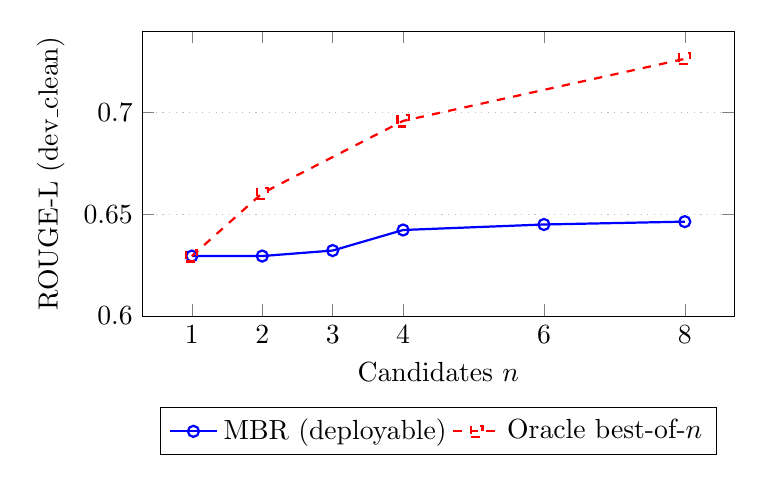
\begin{tikzpicture}
\begin{axis}[width=0.75\linewidth,height=5.2cm,xlabel={Candidates $n$},ylabel={\rl{} (dev\_clean)},legend style={at={(0.5,-0.32)},anchor=north,legend columns=2},ymajorgrids,grid style={dotted},xtick={1,2,3,4,6,8},ymin=0.6,ymax=0.74]
\addplot[mark=o,thick,blue] coordinates {(1,0.6295)(2,0.6295)(3,0.6322)(4,0.6423)(6,0.6450)(8,0.6464)};
\addplot[mark=square,thick,red,dashed] coordinates {(1,0.6295)(2,0.6604)(4,0.6959)(8,0.7264)};
\legend{MBR (deployable),Oracle best-of-$n$}
\end{axis}
\end{tikzpicture}
\caption{MBR recovers only $17\%$ of the gap between greedy ($.630$) and the oracle ($.726$); MBR-4 keeps $\approx\!76\%$ of the MBR-8 gain.}\label{fig:mbrn}
\end{figure}

\paragraph{Post-training ladder.}
Table~\ref{tab:ladder} compares the post-training methods from the same supervised starting point.
\begin{itemize}[leftmargin=*]
\item \textbf{GRPO} moves greedy dev \rl{} by $+0.01$ to $+0.03$, depending on the reward; the final variants span $.612$--$.634$. Started from v3b it does not beat v3b with MBR.
\item \textbf{Merging} the GRPO delta into v3b by task arithmetic matches DPO round~1 under greedy decoding ($+.019$), but its MBR gain is not significant, it needs a GRPO run first, and DPO round~2 is higher. It was not kept.
\item \textbf{On-policy DPO} is the best trade-off. Under \emph{greedy} decoding, round~2 ($.664$) exceeds v3b with MBR-8 ($.658$) at one eighth of the generation cost, and MBR adds only $+0.003$ to $+0.008$ on top of it.
\item \textbf{Round~2 on its own is not significant.} Against round~1 it adds $+.009$ \ci{-.003}{+.023}, which does not pass the acceptance rule. We kept it for three reasons: the two-round chain passes the rule against C1, the round-2 step reproduced with a second DPO seed, and round~2 gained $+.025$ in the first PiSSA chain (Section~\ref{sec:pissa}). It did not help when both rounds were repeated from another SFT seed (below).
\item \textbf{Round~3 over-optimises} (Figure~\ref{fig:dpo}): answers grow to $2{,}000$ characters against a reference mean of $1{,}583$, i.e.\ the policy exploits the lexical reward through length.
\end{itemize}
In the tables, $\mathrm{dpo}_a$ denotes the round-1 model and $\mathrm{dpo}_{a2}$ the round-2 model, i.e.\ the reported system.
\begin{table}[H]
\centering
\caption{Post-training ladder on dev ($n{=}300$, 2 shots, \rl{}). Intervals are paired-bootstrap differences against the row marked $\dagger$ (\ci{lo}{hi}).}\label{tab:ladder}
\begin{tabular}{@{}lccl@{}}
\toprule
System & Greedy & MBR-8 & Difference vs.\ C1 greedy$\dagger$ / C1 MBR-8\\
\midrule
SFT v0 (no shots) & .603 & .637 & MBR $+.034$ \ci{+.020}{+.048}\\
\textbf{C1}: SFT v3b$^\dagger$ & .633 & .658 & MBR $+.025$\\
GRPO, cosine reward (from v0) & .634 & .645 & greedy $+.032$ over v0 \ci{+.019}{+.045}\\
GRPO from v3b & .627 & .651 & $<$C1\\
Task arithmetic v3b + (GRPO$-$v0) & .652 & .667 & +.019 \ci{+.006}{+.034}; MBR $+.009$ (n.s.)\\
DPO round 1 ($\mathrm{dpo}_a$) & .654 & .659 & +.019 \ci{+.001}{+.038}\\
DPO round 1, lr $5\!\times\!10^{-5}$ + SFT term & .642 & .659 & worse than $\mathrm{dpo}_a$\\
\best{DPO round 2 ($\mathrm{dpo}_{a2}$)} & \best{.664} & \best{.672} & \best{+.031 \ci{+.014}{+.049}}; MBR $+.015$ \ci{-.001}{+.030}\\
 & & & vs round 1: $+.009$ \ci{-.003}{+.023} (n.s.)\\
\quad second DPO seed ($\mathrm{dpo}_{a2}'$) & .662 & .665 & +.030 \ci{+.011}{+.050}\\
\quad MBR with 4 candidates & -- & .667 & \\
DPO round 3 ($\mathrm{dpo}_{a3}$) & .635 & .642 & $-.029$ \ci{-.045}{-.012} vs round 2\\
\bottomrule
\end{tabular}
\end{table}
\begin{figure}[H]
\centering
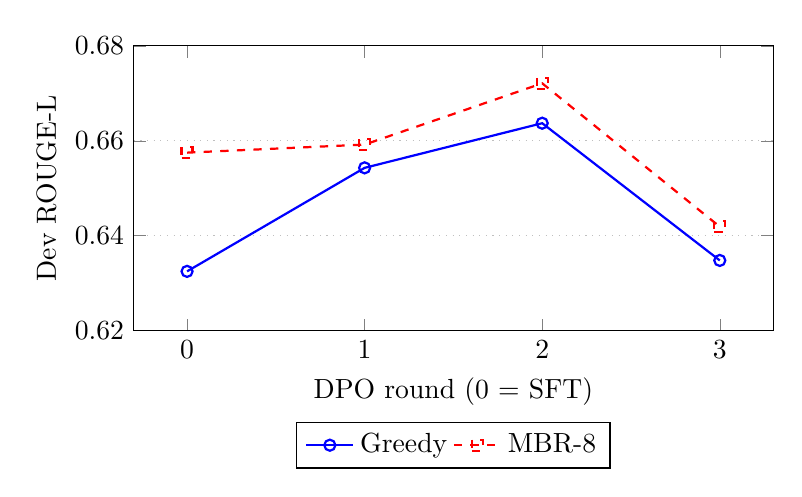
\begin{tikzpicture}
\begin{axis}[width=0.8\linewidth,height=5.2cm,xlabel={DPO round (0 = SFT)},ylabel={Dev \rl{}},legend style={at={(0.5,-0.32)},anchor=north,legend columns=2},ymajorgrids,grid style={dotted},xtick={0,1,2,3},ymin=0.62,ymax=0.68]
\addplot[mark=o,thick,blue] coordinates {(0,0.6325)(1,0.6543)(2,0.6637)(3,0.6348)};
\addplot[mark=square,thick,red,dashed] coordinates {(0,0.6575)(1,0.6592)(2,0.6721)(3,0.6419)};
\legend{Greedy,MBR-8}
\end{axis}
\end{tikzpicture}
\caption{Iterated DPO on self-samples: gains in rounds 1--2, collapse in round 3.}\label{fig:dpo}
\end{figure}

\paragraph{How robust is the DPO gain?}
\begin{itemize}[leftmargin=*]
\item \textbf{Second DPO seed, same supervised model.} Round~2 is reproduced: dev $.6637$ against $.6623$, test $.6433$ against $.6377$.
\item \textbf{Different supervised seeds.} Three SFT seeds on the full data give $.6325$, $.603$ and $.613$ (mean $.616$, standard deviation $.015$). The reported chain starts from the best of the three.
\item \textbf{Repeating both rounds from the $.613$ seed.} Round~1 helps again ($.640$, $+.027$), but round~2 adds nothing ($.634$).
\end{itemize}
The robust effect of on-policy DPO is therefore $+.02$ to $+.03$ over its supervised model. The extra benefit of the second round is real for the reported chain but not guaranteed for another starting seed.

\subsection{Post-training from the PiSSA supervised model}\label{sec:pissa}
The PiSSA adapter gave the best supervised model ($.6414$ dev). We asked whether it, or better preference pairs, could lift the system above $\mathrm{dpo}_{a2}$. Because several of these chains were compared on dev and test, Table~\ref{tab:pissa} reports both splits and their pooled value ($n{=}500$, disjoint questions); test is not an untouched estimate for this comparison. The answer is no. Every round-2 variant except the gold-chosen set ends at a pooled \rl{} of $.647$--$.666$, against $.656$ for $\mathrm{dpo}_{a2}$, and no interval excludes zero in its favour. Whole chains that differ only in the random seed already differ by up to $.019$ ($.6658$ against $.6471$).
\begin{table}[H]
\centering
\caption{Post-training from the PiSSA supervised model $V_p$ (greedy, 2 shots, \rl{}). Pooled = dev$+$test; interval = paired bootstrap against $\mathrm{dpo}_{a2}$. Round~2 always starts from the round-1 model.}\label{tab:pissa}
\footnotesize\setlength{\tabcolsep}{3pt}
\begin{tabular}{@{}lcccl@{}}
\toprule
System & Dev & Test & Pooled & vs.\ $\mathrm{dpo}_{a2}$\\
\midrule
\multicolumn{5}{@{}l}{\emph{Reference and starting points}}\\
$\mathrm{dpo}_{a2}$ (reported system, v3b) & .6637 & .6433 & .6556 & --\\
$V_p$ (PiSSA SFT) & .6414 & .6307 & -- & --\\
$V_p$ + DPO round 1 (two seeds) & .6493 / .6544 & .6226 / .6263 & -- & --\\
\midrule
\multicolumn{5}{@{}l}{\emph{Round 2, standard pairs (the plain recipe)}}\\
chain 1 (two seeds) & .6743 / .6782 & .6435 / .6472 & .6620 / .6658 & $+.006$ / $+.010$ (both n.s.)\\
chain 2 (all steps repeated, other seed) & .6586 & .6299 & .6471 & $-.009$ \ci{-.022}{+.005}\\
round 3 (after chain 1) & .6453 & .6166 & .6338 & $-.022$ \ci{-.035}{-.009}\\
\midrule
\multicolumn{5}{@{}l}{\emph{Round 2, other pair sets}}\\
mixed pairs (two seeds) & .6642 / .6663 & .6418 / .6410 & .6553 / .6561 & $-.000$ / $+.001$\\
mixed $+$ $129$ gold-chosen pairs & .6363 & .6376 & .6368 & $-.019$ \ci{-.033}{-.004}\\
standard $+$ $143$ cite-contrast pairs (two seeds) & .6728 / .6653 & .6413 / .6403 & .6602 / .6553 & $+.005$ / $-.000$\\
\quad same, MBR-8 (first seed) & .6767 & .6465 & .6646 & $+.009$ \ci{-.004}{+.023}\\
$n{=}16$ samples per prompt ($1{,}197$ pairs) & .6589 & .6475 & .6544 & $-.001$ \ci{-.015}{+.012}\\
SFT on own best sample ($921$ rows) instead of DPO & .6546 & .6200 & .6408 & $-.015$ \ci{-.029}{-.000}\\
\bottomrule
\end{tabular}
\end{table}
\begin{itemize}[leftmargin=*]
\item \textbf{PiSSA helps the supervised model, not the final one.} After two DPO rounds its gain over v3b is inside the noise.
\item \textbf{Chains are noisy.} The best chain ($.6743/.6782$ dev) was not reproduced when every step was repeated with another seed ($.6586$).
\item \textbf{A third round hurts again:} dev falls to $.6453$, and answers grow to $1.11\times$ the reference length.
\item \textbf{DPO learns ``shorter''.} In $45$--$55\%$ of the standard pairs the chosen answer is more than $20\%$ shorter than the rejected one, and the number of under-quoting answers on dev rose from $44$ to $52$. A \emph{mixed} set balances both length directions, combining real pairs from the samples with truncated and extended copies (Appendix~\ref{app:failed}). It is stable across seeds (pooled $.6553$ and $.6561$) but not better.
\item \textbf{Pairs must stay on-policy.} Using the reference as the chosen answer for $129$ hard questions loses $.019$. It lowers the share of correctly cited answers ($.741\to.716$) and raises the answers that cite nothing ($3\to8$ of $300$). Fine-tuning on the model's own best sample instead of pairs loses $.015$: the rejected examples carry the signal.
\item \textbf{Targeting the right failure did not help either.} Pairs that contrast a sample citing the gold article with one citing only other articles moved the targeted group ($22$ dev questions) by $+.011$ in one seed and $-.031$ in the other, i.e.\ noise. Doubling the samples per question ($n{=}16$) changed nothing. MBR-8 adds $+.004$/$+.005$.
\end{itemize}

\subsection{Ablations of the final system and of the DPO design}\label{sec:ablation}
Starting from the final system (DPO round~2, greedy, $k{=}5$, $2$ shots, reranker over $50$ dense candidates; dev \rl{} $.6637$), we varied each inference factor alone. Separately, each round-1 DPO training choice was varied against the reference round-1 model ($\mathrm{dpo}_a$, $.6543$). The acceptance rule was fixed beforehand: a change is adopted only if the lower bound of its paired $95\%$ interval on dev is above zero and it is not worse on \texttt{dev\_clean} and \texttt{dev\_strict}. Ties keep the cheaper setting.
\begin{table}[H]
\centering
\caption{One-factor ablations on dev ($n{=}300$, greedy, final model unless stated). Difference against the final system ($.6637$) with a paired-bootstrap interval; $\ast$ = interval excludes zero (worse). $^\dagger$Fine-tuned reranker evaluated on the SFT v3b model, against the stock reranker on that model.}\label{tab:abl}
\begin{tabular}{@{}llcl@{}}
\toprule
Factor & Setting & \rl{} & Difference\\
\midrule
Reranker & none (dense top-5) & .641 & $-.022$ \ci{-.039}{-.006}$^\ast$\\
 & 20 candidates & .663 & $-.001$ \ci{-.012}{+.010}\\
 & 50 candidates (final) & .664 & --\\
 & 100 candidates & .651 & $-.013$ \ci{-.023}{-.003}$^\ast$\\
 & fine-tuned rr (SFT v3b)$^\dagger$ & .625 & $-.007$ vs.\ stock rr (.633)\\
Passages $k$ & 3 & .657 & $-.007$ \ci{-.018}{+.004}\\
 & 5 (final) & .664 & --\\
 & 8 & .666 & $+.002$ \ci{-.010}{+.016} (n.s.)\\
Shots & 0 & .633 & $-.030$ \ci{-.049}{-.013}$^\ast$\\
 & 1 & .656 & $-.008$ \ci{-.023}{+.007}\\
 & 2 (final) & .664 & --\\
 & 3 & .651 & $-.013$ \ci{-.025}{-.002}$^\ast$\\
\midrule
\multicolumn{4}{@{}l}{\emph{DPO round~1 design} (from SFT v3b; reference $\mathrm{dpo}_a$: margin $.1$, $\beta{=}.1$, $.654$)}\\
Pair margin & $0.05$ & .655 & $\approx$ reference\\
 & $0.2$ & .641 & $-.013$ vs.\ reference\\
$\beta$ & $0.05$ & .642 & $-.012$ vs.\ reference\\
 & $0.3$ & .652 & $-.002$ vs.\ reference\\
Anchored pairs & drop chosen $<.5$ & .621 & $-.033$ \ci{-.048}{-.019}$^\ast$\\
 & reference as chosen & .591 & $-.063$ \ci{-.079}{-.047}$^\ast$\\
\bottomrule
\end{tabular}
\end{table}
No single factor improves on the final configuration:
\begin{itemize}[leftmargin=*]
\item the reranker over $50$ candidates, $k{=}5$ and two shots are at or near the optimum;
\item removing the reranker costs $0.022$;
\item the only nominally better setting, $k{=}8$ ($+.002$), is not significant and lengthens the context, so it is not adopted;
\item no DPO design variant exceeds the reference margin and $\beta$ ($0.1$/$0.1$);
\item \emph{anchored} pairs, which never teach a chosen answer below \rl{} $0.5$, are clearly worse. In $19\%$ of the round-1 pairs ($227$ of $1{,}211$) the chosen answer scores below $0.5$, because when all $8$ samples are poor the best of them is poor too. Dropping these pairs ($984$ left) loses $.033$. Keeping the $984$ pairs and, for the $257$ prompts whose best sample is below $0.5$ (with or without a standard pair), using the reference as chosen against the worst sample (plus an SFT term of weight $0.2$) loses $.063$. Both models over-lengthen: median answers of $1{,}863$ and $2{,}148$ characters against $1{,}563$ for $\mathrm{dpo}_a$ and a reference mean of $1{,}583$. A low-scoring pair still teaches the model to avoid the worse answer, and it also balances the length direction of the pairs.
\end{itemize}
Because the per-factor winners coincide with the final configuration, the best combined configuration \emph{is} the final system.

\subsection{A configuration fixed in advance, trained on train and dev}\label{sec:finalchain}
The comparisons above select on dev, and the PiSSA comparisons also looked at test. As a last check we fixed one configuration before training and scored it on test once per decoding mode:
\begin{enumerate}[leftmargin=*]
\item supervised fine-tuning on train \emph{and} dev ($1{,}640$ decontaminated rows; PiSSA, rank $32$, three epochs);
\item a first DPO round on $8$ on-policy samples with the standard pairs;
\item a second round with the mixed pair set;
\item greedy decoding and MBR-8.
\end{enumerate}
Only one chain (seed $1$) was trained, so the seed spread of up to $.019$ applies to its number. Since test had already been used to compare the PiSSA recipes, this is not an untouched estimate either.
\begin{table}[H]
\centering\small
\caption{Configuration fixed in advance, trained on train$+$dev, scored once on test ($n{=}200$), next to the reported system.}\label{tab:finalchain}
\begin{tabular}{lccccc}
\toprule
Model and decoding & Cosine & Jaccard & Token overlap & BLEU-1 & \rl{} \\
\midrule
Fixed configuration (train+dev), greedy & .919 & .675 & .729 & .586 & .640 \\
Fixed configuration (train+dev), MBR-8 & .921 & .681 & .718 & .579 & .646 \\
Reported system, greedy & .916 & .673 & .734 & .582 & .643 \\
Reported system, MBR-8 & .918 & .681 & .728 & .587 & .652 \\
\bottomrule
\end{tabular}
\end{table}
\noindent Adding dev to the training data does not move test: both differences ($-.003$ greedy, $-.006$ MBR-8) are well inside the seed spread, as the learning curve predicted ($\approx+.003$). The reported system therefore stays the first recipe (v3b with two DPO rounds).

%------------------------------------------------------------------------------
\section{Analysis}\label{sec:analysis}
\subsection{Where the error is}\label{sec:where}
For the supervised model (v0) on dev, the score depends mostly on whether the gold \dieu{} is both retrieved and cited:

\begin{center}
\small
\begin{tabular}{@{}lcc@{}}
\toprule
Gold \dieu{} & Questions & \rl{}\\
\midrule
retrieved and cited & $205$ & $.702$\\
retrieved, another article cited & $28$ & $.397$\\
not retrieved & $25$ & $.295$\\
\bottomrule
\end{tabular}
\end{center}

\noindent Over the $281$ dev questions whose reference cites an article, the model cites the same article in $68.3\%$ of cases (v3b) and $70.5\%$ (round-1 DPO). Answers score $.73$--$.76$ when the citation matches and $.43$--$.46$ when it does not.

For the final model on dev (mean $.664$), the scores split into three groups:
\begin{itemize}[leftmargin=*]
\item \textbf{High}, $34\%$ of answers, scoring $\ge.8$ (mean $.91$);
\item \textbf{Middle}, $48\%$, scoring $.4$--$.8$ (mean $.63$); this group holds $54\%$ of the distance to $1.0$;
\item \textbf{Tail}, $17\%$, scoring below $.4$ (mean $.28$); this group holds $37\%$.
\end{itemize}
Among the questions whose reference cites an article, the answer names that article in only $18$ of $40$ in the tail, against $112$ of $128$ in the middle and $95$ of $96$ in the high group. The typical failure is the right law with a neighbouring article, or a different law that also fits an under-specified question.

\paragraph{Length.}
Overall length was a problem before DPO and matches the reference after it. For the SFT model, predicted answers had a median of $315$ words against $294$ for the reference, and truncating them to the reference length would have added $+0.028$. After DPO, the median lengths match ($292$ against $294$ words), longest-common-subsequence precision and recall are about equal in every group, and the best truncation adds only $+0.0006$. Per answer, however, DPO pairs favour the shorter answer, and a few more answers under-quote (Section~\ref{sec:pissa}).

\paragraph{Headroom.}
Three oracles bound what selection could still gain:
\begin{itemize}[leftmargin=*]
\item \textbf{Best of $8$ samples}, picked with knowledge of the reference: $.726$ on \texttt{dev\_clean}, $0.08$ above MBR.
\item \textbf{The better of the model answer and a verbatim quotation of the gold article}, chosen per question: dev reaches $.722$ ($+.059$; $+.032$ from the middle group and $+.025$ from the tail).
\item \textbf{The same using only what is available at inference} (the answer and a quotation of each of the five retrieved passages): $.715$.
\end{itemize}
The tail would rise only from $.28$ to $.42$, because references also contain text that is not in the article. A learned selector over the same six candidates reaches $.644$ (5-fold cross-validation on dev), below the model alone. We found no deployable selector that captures this headroom.

\subsection{Is model size the limit? A 4B and a 9B scaling point}\label{sec:scaling}
To separate model size from data and clause choice, we re-ran the reported recipe unchanged on Qwen3.5-4B ($4.66$B) and Qwen3.5-9B ($9.65$B). The recipe is SFT v3b followed by two on-policy DPO rounds, with the same data, hyper-parameters, retrieval and shots. Dev was scored after every stage, and test once at the end per decoding mode. Both models exceed the 4B limit, so they are analysis only and not candidates for the submitted system.

\begin{table}[H]
\centering\small
\caption{Scaling the reported recipe (\rl{}). Dev $n{=}300$, test $n{=}200$; greedy unless stated.}\label{tab:scaling}
\begin{tabular}{@{}lccccccc@{}}
\toprule
Base model & Params & SFT & DPO r1 & DPO r2 & Dev MBR-8 & Test & Test MBR-8\\
\midrule
\best{Qwen3.5-2B (reported)} & \best{2.27B} & \best{.633} & \best{.654} & \best{.664} & \best{.672} & \best{.643} & \best{.652}\\
Qwen3.5-4B & 4.66B & .636 & .669 & .679 & .686 & .666 & .672\\
Qwen3.5-9B & 9.65B & .664 & .693 & .700 & .705 & .677 & .686\\
\bottomrule
\end{tabular}
\end{table}
\begin{itemize}[leftmargin=*]
\item \textbf{Size helps, but little.} About $4\times$ the parameters add $.034$ test \rl{} ($.643\to.677$); 4B adds $.023$. This is about the gain of one DPO round, and less than twice the spread between seeds ($.019$).
\item \textbf{The recipe transfers.} Two DPO rounds add $+.031$ to $+.043$ on dev at every size ($+.031$, $+.043$, $+.036$), so its gain is not specific to the 2B model.
\item \textbf{Most of the gap opens in post-training.} After SFT the 4B model is level with the 2B ($.636$ against $.633$). Only the 9B starts higher ($.664$, the level the 2B reaches after two DPO rounds).
\item \textbf{A larger model chooses clauses somewhat better.} On dev the 9B ($.700$) recovers about $60\%$ of the gap between the 2B ($.664$) and the oracle that picks, per question, the better of the answer and a verbatim gold quotation ($.722$, Section~\ref{sec:where}). This is consistent with part of the remaining error being a matter of capacity, but it does not isolate clause choice, since that oracle is built from the 2B's answers. The price is $4\times$ the parameters for $+.034$ on test, and no model inside the 4B limit is available to buy it. Within the limit, the 2B system is close to what this recipe can reach.
\end{itemize}

\subsection{Why DPO on self-samples works here}
\begin{itemize}[leftmargin=*]
\item The reward is the evaluation metric.
\item The pairs are on-policy, so there is no shift between the sampled model and the trained one.
\item The gap threshold removes noisy pairs.
\end{itemize}
Reaching the best of $8$ samples in a single pass is the same objective that MBR pursues at inference time. The failure of round~3, and of off-policy chosen answers, marks the two limits: the policy starts to exploit the lexical reward through length, and text the model would not generate itself carries no usable contrast.

\subsection{What can be checked automatically}
Legal validity, and whether a provision is still in force, cannot be judged without a legal expert. Three properties can be measured without one (Table~\ref{tab:checks}):
\begin{itemize}[leftmargin=*]
\item \textbf{Citation agreement.} On test, $67\%$ of answers cite \emph{every} article that the reference cites, and $78\%$ name a legal document that the reference names. Roughly a third of the answers miss at least one reference article; this is the main error type.
\item \textbf{Numbers are rarely invented.} $96.5\%$ of the numeric tokens in the answers occur in the retrieved passages or in the question, and $88\%$ of the answers that contain numbers are fully grounded. The references themselves are grounded at $90.7\%$, since they sometimes use information outside the retrieved texts.
\item \textbf{Quotation.} Answers reproduce $66\%$ of their 8-grams verbatim from the sources, against $55\%$ for the references: the model quotes more than the annotators did.
\end{itemize}
Worked examples ordered from easy to hard are given in Appendix~\ref{app:examples}.
\begin{table}[H]
\centering
\caption{Automatic checks of the final system's test answers ($n{=}200$). Agreement rates are over the questions whose reference contains an article or a law identifier; grounding is over the answers that contain numbers.}\label{tab:checks}
\begin{tabular}{@{}lcc@{}}
\toprule
Check & System answers & References (context)\\
\midrule
Cites every article cited by the reference & .670 & --\\
Names a legal document named by the reference & .782 & --\\
Numeric tokens found in sources or question (mean) & .965 & .907\\
Answers whose numbers are all grounded & .880 & --\\
8-gram quotation rate from the retrieved passages & .664 & .546\\
\bottomrule
\end{tabular}
\end{table}

\subsection{What did not help}\label{sec:negative}
Table~\ref{tab:neg} collects every idea that was tested and not kept, grouped by pipeline stage. Appendix~\ref{app:failed} gives the details of the post-training and weight-editing attempts.
\begin{table}[H]
\centering
\caption{Ideas tested and not retained (greedy dev \rl{} unless stated; reference: the final system, $.6637$, or the stated baseline).}\label{tab:neg}
\small\setlength{\tabcolsep}{4pt}
\begin{tabular}{@{}>{\raggedright\arraybackslash}p{5.2cm}>{\raggedright\arraybackslash}p{4.4cm}>{\raggedright\arraybackslash}p{5.6cm}@{}}
\toprule
Idea & Result & Why it did not help\\
\midrule
\multicolumn{3}{@{}l}{\emph{Retrieval}}\\
Fine-tuned reranker / embedder & \dieu{}@1 $+.12$ / $+.023$; generation $.6325\to.6253$ & Ranking gains do not reach the answer\\
Hybrid BM25 + dense & on par after reranking & Lexical recall is far weaker\\
Other chunkings (5 variants) & \dieu{}@5 $-.023$ to $+.004$ & Per-article chunks are already the natural unit\\
LLM re-ranking (GLM-5.3, DeepSeek-V4) & \dieu{}@1 $+.14$/$+.10$; \rl{} $+.002$/$0$ & The model does not use a better order\\
$k{=}10$ passages & $.612$ vs $.633$ (v3b) & Longer context dilutes the gold passage\\
\midrule
\multicolumn{3}{@{}l}{\emph{Generator}}\\
Legal-domain base model (3B) & $.615$ vs $.633$ after SFT & Knowledge comes from retrieval\\
Continued pre-training (209M tokens) & cloze $+15$ points, \rl{} unchanged & Extent and style, not knowledge, limit \rl{}\\
Distillation \cite{hinton} from a 9B teacher & raw teacher $.41$--$.43$ $<$ SFT 2B & Teacher does not follow the reference register\\
Thinking at inference / thinking SFT on rationales & $.590$ vs $.603$ / $.585$ vs $.641$ & Reasoning does not make the quotation more accurate (Table~\ref{tab:think})\\
\midrule
\multicolumn{3}{@{}l}{\emph{Post-training}}\\
GRPO from v3b & $.627$ vs $.633$ & DPO on self-samples is better and cheaper\\
Task arithmetic, v3b + GRPO delta & $.652$ vs $.633$; MBR gain n.s. & Needs a GRPO run; DPO round~2 is higher\\
Third DPO round & $-.029$ (v3b chain), $-.022$ pooled (PiSSA) & Exploits the reward through length\\
Gold answers as chosen / own best sample as SFT target & $-.019$ / $-.015$ pooled & Off-policy text, or no rejected examples\\
Higher cited-article weight in the reward ($0.4$/$0.6$) & $.6551$ / $.6458$ vs $.6543$ & No gain at round~1\\
Anchored pairs: drop chosen $<.5$ / reference as chosen & $.621$ / $.591$ vs $.654$ & Loses the ``avoid worse'' signal; answers grow longer\\
Cite-contrast, $n{=}16$, length-balanced pairs & $-.001$ to $+.005$ pooled & Inside the seed spread\\
Averaging two DPO seeds; agent edits of the weights & no gain; best $+.004\pm.005$ & Remaining loss is question-specific\\
\midrule
\multicolumn{3}{@{}l}{\emph{Decoding and post-processing}}\\
Truncate long answers; convert tone-mark style & $+.0006$ / $-.0017$ & Length and spelling already match\\
Replace the quotation by the whole article & $-.085$ & References quote only part of it\\
Quote the rank-1 passage / MBR over \{answer, quotes\} & $.534$ / $.557$ & Loses the template and the right clause\\
Learned selector over \{answer, 5 quotes\} & $.644$ (oracle $.715$) & Cannot tell which clause is right\\
Complete a partly quoted clause by rule & $-.002$ to $-.006$ & The reference also quotes only part of a list\\
Clause hint from lexical overlap & right at rank one $21\%$ vs model $52\%$ & The model chooses the clause better\\
Cascade: MBR only if uncertain & $.644$ at $3.1$ generations (MBR-8 $.658$) & Reranker margin weakly predicts MBR gain\\
FP8 weights & $.646$ vs $.654$ ($-.009$ \ci{-.020}{+.002}) & $21\%$ lower latency is not worth the loss\\
\midrule
\multicolumn{3}{@{}l}{\emph{Agents}}\\
ReAct agent \cite{react} with 4 tools (search, article, graph, web) & \texttt{dev\_clean} $.537$--$.574$ vs $.634$ (v3b, same subset); $-0.060$ \ci{-0.097}{-0.026} & Own queries find the gold article in only $66$--$72\%$ of questions\\
\bottomrule
\end{tabular}
\end{table}

%------------------------------------------------------------------------------
\section{Deployment}\label{sec:deploy}
\subsection{Service}
The final configuration is packaged as a docker-compose stack:
\begin{itemize}[leftmargin=*]
\item three vLLM v0.30.0 endpoints, for the DPO model in bf16, the embedder and the reranker (GPU memory fractions $.45/.15/.15$ of one L40S; the single-card load tests in Section~\ref{sec:capacity} give the LLM $.60$);
\item an API image ($0.7$\,GB, no model weights) that holds the $12.4$\,GB index in RAM and the few-shot pool as a $3$\,MB JSON file.
\end{itemize}
The service exposes \texttt{POST /ask} (also streaming, as server-sent events and an OpenAI-compatible chat-completions endpoint) and \texttt{GET /health}. It returns the answer, the five reranked sources and per-stage timings. It exposes Prometheus metrics, can bound the number of running and queued requests (HTTP~429 beyond the queue), and is configured by environment variables so that the same image can call shared endpoints.

\paragraph{Refusal guard.} When the best reranker score is below $\tau{=}0.001$ (no corpus support), the service answers with a fixed refusal sentence without calling the LLM. Only $4$ of $300$ dev questions fall below $\tau$.

\begin{table}[H]
\centering
\caption{Measured behaviour through the HTTP API (dev questions, greedy, $k{=}5$, 2 shots). The \rl{} values are parity checks on few questions only.}\label{tab:lat}
\begin{tabular}{@{}lccccc@{}}
\toprule
Setting & $n$ & \rl{} & Mean & p50 & p95\\
\midrule
1 request at a time & 25 & .674 & 3.15\,s & 2.61\,s & 6.61\,s\\
4 concurrent requests & 30 & .703 & 4.36\,s & 3.51\,s & 9.65\,s\\
\bottomrule
\end{tabular}
\end{table}
For a single request, the mean time per stage is $0.08$\,s for retrieval, $0.21$\,s for reranking and $2.85$\,s for generation ($91\%$), so decoding dominates.

\paragraph{Demonstration.}
Ten questions were sent to the live service (transcript in \texttt{docs/report/demo.md}):
\begin{itemize}[leftmargin=*]
\item \textbf{Six development questions} with references: \rl{} $.558,.617,.753,.601,.675,.821$ (mean $.671$).
\item \textbf{Three free questions} (traffic fines, personal income tax deductions, capital adequacy ratio). For the traffic question the system answers in the reference register (``\textit{Căn cứ theo khoản 1 Điều 6 Nghị định 100/2019/NĐ-CP được sửa đổi bởi \ldots}'') and quotes the retrieved article. We did not verify its legal validity, and the retrieved text may predate later amendments: the metric rewards similarity to references, not legal correctness.
\item \textbf{One off-topic question} (``weather in Hanoi''). Its first run exposed a failure: the model invented a repeating weather bulletin while every reranker score was $0.000$. This motivated the refusal guard, and the service now refuses in $0.3$\,s.
\end{itemize}

\subsection{Capacity under concurrent load and GPU layout}\label{sec:capacity}
We measured three layouts on the two L40S cards:
\begin{itemize}[leftmargin=*]
\item \textbf{A$'$}: one card, everything shared (LLM $60\%$ of memory; the baseline);
\item \textbf{B}: one complete stack per card (LLM, embedder, reranker, API) behind an nginx least-connections balancer;
\item \textbf{C}: the LLM alone on card~0, embedder and reranker on card~1.
\end{itemize}
The load generator is closed-loop: each virtual user sends dev questions back to back for $30$\,s, and times are measured client-side through the streaming endpoint. GPU utilisation and temperature are sampled every second, and a run stops at $85^\circ$C. The target is the $95$th percentile of total latency; $p_{99}$ is shown beside it.

The first load test exposed a defect that unit tests had missed. Under concurrent requests, dozens of fresh threads calling FAISS made OpenBLAS raise ``too many memory regions'', and the API process aborted. Retrieval now runs on a bounded thread pool with one BLAS thread each, and every run below has zero errors and zero API restarts.
\begin{table}[H]
\centering
\caption{Closed-loop sweep (dev questions, $n$ users, $30$\,s per level). req/s = completed requests per second; latencies are end-to-end seconds.}\label{tab:capacity}
\small\setlength{\tabcolsep}{3.5pt}
\begin{tabular}{@{}rccccccccc@{}}
\toprule
 & \multicolumn{3}{c}{A$'$ (1 card)} & \multicolumn{3}{c}{B (2 cards, replicas)} & \multicolumn{3}{c}{C (2 cards, split)}\\
\cmidrule(lr){2-4}\cmidrule(lr){5-7}\cmidrule(lr){8-10}
users & req/s & $p_{95}$ & $p_{99}$ & req/s & $p_{95}$ & $p_{99}$ & req/s & $p_{95}$ & $p_{99}$\\
\midrule
1 & .26 & 6.9 & 6.9 & .26 & 7.0 & 7.0 & .26 & 7.0 & 7.0\\
4 & .89 & 8.9 & 9.6 & 1.07 & 7.9 & 7.9 & 1.05 & 8.2 & 8.6\\
8 & 1.59 & 11.0 & 11.2 & 1.85 & 8.7 & 9.3 & 1.84 & 9.2 & 9.9\\
16 & 2.43 & 14.6 & 15.7 & 2.87 & 11.3 & 11.7 & 2.87 & 11.1 & 11.8\\
32 & 3.07 & 19.7 & 24.4 & 4.65 & 12.7 & 16.2 & 4.61 & 12.9 & 15.6\\
64 & 3.48 & 30.9 & 33.9 & 5.76 & 18.4 & 25.3 & 5.63 & 18.5 & 22.4\\
\bottomrule
\end{tabular}
\end{table}
\begin{figure}[H]
\centering
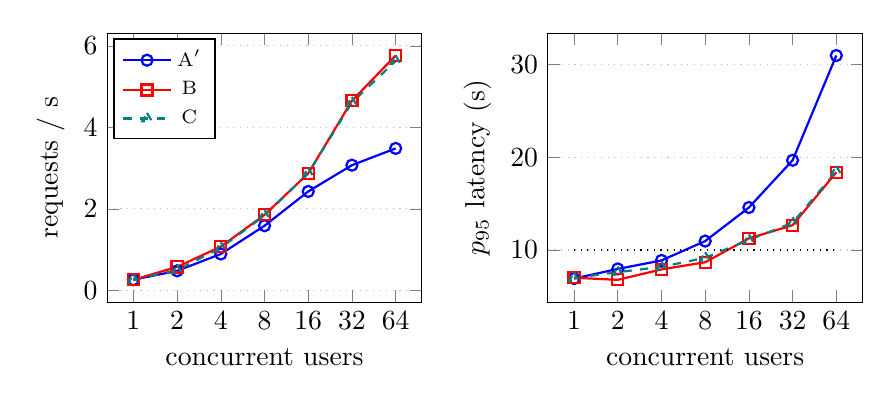
\begin{tikzpicture}
\begin{groupplot}[group style={group size=2 by 1,horizontal sep=1.6cm},width=0.46\linewidth,height=5cm,xmode=log,log basis x=2,xtick={1,2,4,8,16,32,64},xticklabels={1,2,4,8,16,32,64},ymajorgrids,grid style={dotted},xlabel={concurrent users}]
\nextgroupplot[ylabel={requests / s},legend style={at={(0.02,0.98)},anchor=north west,font=\scriptsize}]
\addplot[mark=o,thick,blue] coordinates {(1,.262)(2,.48)(4,.893)(8,1.586)(16,2.427)(32,3.072)(64,3.483)};
\addplot[mark=square,thick,red] coordinates {(1,.259)(2,.577)(4,1.074)(8,1.853)(16,2.871)(32,4.652)(64,5.762)};
\addplot[mark=triangle,thick,teal,dashed] coordinates {(1,.262)(2,.496)(4,1.048)(8,1.837)(16,2.872)(32,4.61)(64,5.628)};
\legend{A$'$,B,C}
\nextgroupplot[ylabel={$p_{95}$ latency (s)}]
\addplot[mark=o,thick,blue] coordinates {(1,6.923)(2,7.962)(4,8.876)(8,10.962)(16,14.576)(32,19.664)(64,30.946)};
\addplot[mark=square,thick,red] coordinates {(1,7.013)(2,6.789)(4,7.909)(8,8.687)(16,11.251)(32,12.669)(64,18.368)};
\addplot[mark=triangle,thick,teal,dashed] coordinates {(1,6.978)(2,7.619)(4,8.178)(8,9.164)(16,11.086)(32,12.933)(64,18.461)};
\addplot[black,dotted] coordinates {(1,10)(64,10)};
\end{groupplot}
\end{tikzpicture}
\caption{Throughput and $p_{95}$ latency versus concurrent users; the dotted line is the $10$\,s target.}\label{fig:capacity}
\end{figure}
\paragraph{Maximum concurrency.} We define it as the largest number of users that keeps $p_{95}<10$\,s with no error and no rejection, found by doubling and then bisecting.

\begin{center}
\small
\begin{tabular}{@{}lc@{}}
\toprule
Layout & Maximum users\\
\midrule
A$'$ (one card) & $6$--$7$ (two settings of the LLM memory share)\\
B (two replicas) & $15$ and $18$ (two independent measurements)\\
C (split) & $18$\\
\bottomrule
\end{tabular}
\end{center}

\noindent Two cards thus serve about $2.5$ to $3\times$ as many users as one. B and C cannot be told apart in capacity, but C keeps the second card at only $25$--$50\%$ utilisation. We keep B as the default because the replicas fail independently (the balancer routes around a dead stack); C is the choice when the second card is shared with other work.

\paragraph{Bursts.} Every layout served all requests without errors in both burst tests.
\begin{itemize}[leftmargin=*]
\item \textbf{Open-loop run} (Poisson arrivals at $0.5$\,req/s, then $4$\,req/s for $15$\,s, then $0.5$\,req/s). The $p_{95}$ during the burst was $12.2$\,s on one card, against $9.0$\,s (B) and $9.2$\,s (C). After the burst, the $p_{95}$ returned to $0.86$--$0.92$ of its pre-burst value.
\item \textbf{$64$ requests released at once.} Draining them took $22.1$\,s on one card, $15.4$\,s (B) and $16.4$\,s (C).
\end{itemize}
Each level contains only $8$ to $220$ requests, so $p_{99}$ is close to the maximum and noisy. Repeated measurements for B agree within about $0.3$\,s at $p_{95}$, except near the threshold.

\paragraph{Engine settings.} On the single-card layout we varied the vLLM settings one at a time (Table~\ref{tab:flags}; no errors in any run):
\begin{itemize}[leftmargin=*]
\item \textbf{Scheduling limits do not matter.} The number of concurrently decoded sequences ($32$--$256$) and the per-step token budget ($8$k--$32$k) change nothing beyond run-to-run noise: decoding, not scheduling, saturates the card.
\item \textbf{FP8 key--value cache} gives the same throughput at lower memory use; the context is short, so the saved memory is not needed.
\item \textbf{Prefix caching should stay on.} Disabling it lowers throughput at $32$ users by about $9\%$ ($2.70$ against $2.98$\,req/s) and lengthens the tail, because every request shares the instruction and the two demonstrations as a common prefix.
\end{itemize}
The defaults of the deployed stack are therefore unchanged.
\begin{table}[H]
\centering
\caption{vLLM settings on one card (layout A$'$), requests/s and $p_{95}$ latency (s) at $16$ and $32$ concurrent users. $^\dagger$64 sequences, 16k batched tokens, prefix caching on.}\label{tab:flags}
\small\setlength{\tabcolsep}{4pt}
\begin{tabular}{@{}lcccc@{}}
\toprule
 & \multicolumn{2}{c}{16 users} & \multicolumn{2}{c}{32 users}\\
\cmidrule(lr){2-3}\cmidrule(lr){4-5}
Setting & req/s & $p_{95}$ & req/s & $p_{95}$\\
\midrule
default$^\dagger$ & 2.20 & 16.3 & 2.98 & 19.7\\
32 / 128 / 256 sequences & 2.24 / 2.22 / 2.24 & 15.4 / 16.0 / 16.1 & 2.98 / 3.03 / 3.02 & 18.9 / 19.0 / 18.8\\
8k / 32k batched tokens & 2.20 / 2.21 & 16.3 / 16.2 & 3.00 / 3.02 & 19.3 / 19.2\\
no prefix caching & 2.26 & 14.6 & 2.70 & 21.1\\
FP8 KV cache & 2.14 & 16.2 & 2.99 & 20.6\\
\bottomrule
\end{tabular}
\end{table}

\subsection{Speculative decoding (exploratory)}\label{sec:spec}
Answers quote the passages in the prompt, so n-gram prompt lookup \cite{vllm} could propose many tokens for free. We served a 2B model of the PiSSA chain (same architecture as the deployed one) on one card and generated $40$ dev answers per setting (Table~\ref{tab:spec}).
\begin{itemize}[leftmargin=*]
\item \textbf{One request at a time:} decoding becomes $1.5$--$2.4\times$ faster, and $p_{95}$ drops from $6.2$\,s to $2.4$\,s with $8$ proposed tokens.
\item \textbf{$16$ concurrent requests:} throughput falls to $0.52$--$0.95\times$, because the card is already saturated and rejected proposals waste compute.
\item \textbf{Correctness not established:} only $11$--$15$ of the $40$ answers were identical to plain decoding, although speculative decoding should not change greedy output. Until that is explained, it is not part of the deployed stack.
\end{itemize}
\begin{table}[H]
\centering
\caption{N-gram speculative decoding, generated tokens per second (speed-up against no speculation), $40$ dev prompts.}\label{tab:spec}
\small
\begin{tabular}{@{}lcc@{}}
\toprule
Proposed tokens (lookup window) & 1 request & 16 concurrent\\
\midrule
none & 160 & 1380\\
3 (2--3) & 242 ($1.51\times$) & 722 ($0.52\times$)\\
5 (2--4) & 312 ($1.95\times$) & 1099 ($0.80\times$)\\
8 (2--5) & 382 ($2.39\times$) & 1305 ($0.95\times$)\\
\bottomrule
\end{tabular}
\end{table}

%------------------------------------------------------------------------------
\section{Limitations and Threats to Validity}\label{sec:limits}
\begin{itemize}[leftmargin=*]
\item \textbf{Selection on dev.} Up to about ten variants were compared at several stages on a $300$-question dev set. Intervals are paired but not corrected for multiple comparisons, and the \texttt{dev\_clean} ($166$) and \texttt{dev\_strict} ($74$) subsets are small.
\item \textbf{Seed dependence.} The reported chain starts from the best of three SFT seeds, so its absolute dev level ($.664$) is optimistic by a few hundredths. Whole chains differing only in the seed differ by up to $.019$ \rl{} (pooled), as much as most claimed gains. Round~2 DPO was reproduced with a second DPO seed on the same supervised model, but not from another supervised seed.
\item \textbf{Use of test.} Test was scored for earlier configurations (not used for selection), used together with dev to compare the PiSSA recipes, scored once for the configuration fixed in advance, and scored once per decoding mode for the 4B/9B scaling points (analysis only). Retrieval tables show test numbers next to dev; they were not used for selection. Test differences below $\approx0.02$ are within bootstrap noise.
\item \textbf{Reference-style metric.} All metrics measure lexical or embedding similarity to references written in a fixed template. They do not measure legal correctness, and they favour models fine-tuned on the same template. Train and test answers share $13$-grams in $32\%$ of test questions.
\item \textbf{Retrieval store.} The index was extended with laws that the QA set cites; the protocol permits this, since the store may hold laws but no test QA pairs. Law-hit is $0.62$ on test. For the remaining questions, including those without an extractable law identifier, the answer must rely on related passages.
\item \textbf{Non-determinism.} Identical vLLM runs differ by $\pm0.003$ \rl{} with greedy decoding and by $\pm0.006$ with MBR.
\item \textbf{Legal validity.} Answers are generated from retrieved texts that may be outdated or superseded and are not legal advice; legal experts did not assess correctness. The automatic checks of Table~\ref{tab:checks} cover only citation agreement and faithfulness to the retrieved text, not currency or legal soundness.
\item \textbf{Load tests.} Capacity was measured with synthetic closed-loop and burst traffic made of dev questions, on a machine shared with other users' jobs. No real user traffic was observed. The speculative-decoding test covers $40$ prompts and changed the greedy output.
\end{itemize}

\section{Future Work}\label{sec:future}
The following directions were not run. For each we state the protocol under which it would be tested and the effect we expect.

\paragraph{Choosing the clause, not the article.}
The remaining error is mostly which \textit{khoản} is quoted and how much of it. The oracle quotations show $+.05$--$.06$ of headroom; a lexical hint and a learned selector did not capture it. A small cross-encoder trained to score (question, \textit{khoản}) pairs on the training references could supply a ranked clause list to the prompt or to a selector over samples. It would be judged on dev \rl{} with the usual bootstrap, and on whether it beats the model's own clause choice ($52\%$ at rank one).

\paragraph{A checker for selection and abstention.}
Retrieval-side critics such as Self-RAG \cite{selfrag} and Corrective RAG \cite{crag} report gains in accuracy and citation precision. However, the only lexical-overlap result we found (Self-RAG on ASQA: ROUGE $35.7$ against $35.8$ for a plain fine-tuned model) shows no change, and self-correction without reliable external feedback tends to hurt smaller models \cite{selfcorrect,kamoi}. A claim-level verifier for Vietnamese labour-law QA improved citation preservation by only $+0.02$ to $+0.03$ \cite{nllp26}. We therefore expect a frozen sub-4B verifier to improve citation agreement and grounding (Table~\ref{tab:checks}) rather than \rl{}. Proposed protocol:
\begin{enumerate}[leftmargin=*,label=(\roman*)]
\item \emph{selection}: choose among the $8$ samples that MBR already scores, compared with MBR and with the best-of-$8$ oracle;
\item \emph{abstention}: gate answers that the retrieved articles do not support, replacing the reranker-score guard;
\item no rewriting step.
\end{enumerate}

\paragraph{Length-controlled preference rewards.}
Round~3 of DPO fails by lengthening answers, and the standard pairs favour shorter answers. A reward with an explicit length term relative to the reference, or a length-normalised objective \cite{simpo}, could allow a third round without collapse. It would be tested on two seeds against the round-2 model.

\paragraph{Speculative decoding for single users.}
Before n-gram speculation is used to cut single-user latency by up to $2.4\times$, its outputs must be shown to equal plain greedy decoding on the full dev set. The mismatch observed on $40$ prompts must be traced first.

\section{Conclusion}
A $2.27$B model reaches test \rl{} $0.643$ with a single generation per question ($0.652$ with MBR-8), up from $0.171$ for the course baseline. It combines a well-covered index, a supervised recipe that teaches the answer register, and two rounds of on-policy DPO on its own best-versus-worst samples. The decisive factors are, in order:
\begin{enumerate}[leftmargin=*]
\item \emph{retrieval coverage};
\item \emph{supervised register learning};
\item \emph{metric-aligned preference optimisation}.
\end{enumerate}
A second adapter recipe (PiSSA), several new pair sets and a configuration fixed in advance and trained on train plus dev all land within the seed spread of this system ($0.640$/$0.646$ for the latter). This suggests the recipe is at its limit with the available data. Model size helps, but only a little. The same recipe on Qwen3.5-4B and 9B, both beyond the 4B rule and run as analysis only, reaches test $0.666$ and $0.677$, only $+0.02$ to $+0.03$ above the 2B system. None of the following improved the score:
\begin{itemize}[leftmargin=*]
\item additional retrieval training;
\item legal-domain base models and continued pre-training;
\item thinking-mode training;
\item agents;
\item quantisation.
\end{itemize}
What remains is the choice of clause and of quotation extent, which no deployable selector has yet captured. The system runs as a containerised service: one L40S serves $6$--$7$ concurrent users and two serve $15$--$18$ within a $10$\,s p95.

\section*{Reproducibility}
Code, configurations, the container stack and a step-by-step manual are in the repository (\texttt{README.md}, \texttt{docs/ops/docker.md}). Every number above corresponds to a run directory with its configuration and predictions; the experiment log is in \texttt{docs/CHANGELOG.md}. Code: \url{https://github.com/hoangphu7122002/law-rag}. Data and weights are on the Hugging Face Hub, account \href{https://huggingface.co/hoangphu7122002ai}{\texttt{hoangphu7122002ai}} (all models merged, bf16, same prompt):

\begin{center}\small
\begin{tabular}{@{}lll@{}}
\toprule
Artifact & Repository & Dev / test\\
\midrule
Corpus snapshot, split, SFT and DPO data & \href{https://huggingface.co/datasets/hoangphu7122002ai/law-rag-data}{\texttt{law-rag-data}} & --\\
\textbf{Reported system} (SFT v3b + 2 DPO rounds) & \href{https://huggingface.co/hoangphu7122002ai/law-rag-qwen3.5-2b-dpo}{\texttt{law-rag-qwen3.5-2b-dpo}} & \textbf{.664 / .643}\\
SFT v3b (its supervised stage) & \href{https://huggingface.co/hoangphu7122002ai/law-rag-qwen3.5-2b-sft}{\texttt{law-rag-qwen3.5-2b-sft}} & .633 / .607\\
PiSSA SFT (best supervised model) & \href{https://huggingface.co/hoangphu7122002ai/law-rag-qwen3.5-2b-pissa-sft}{\texttt{law-rag-qwen3.5-2b-pissa-sft}} & .641 / .631\\
Fixed configuration, train+dev: SFT & \href{https://huggingface.co/hoangphu7122002ai/law-rag-qwen3.5-2b-trainval-sft}{\texttt{law-rag-qwen3.5-2b-trainval-sft}} & -- / --\\
\quad + DPO round 1 & \href{https://huggingface.co/hoangphu7122002ai/law-rag-qwen3.5-2b-trainval-dpo1}{\texttt{law-rag-qwen3.5-2b-trainval-dpo1}} & -- / --\\
\quad + DPO round 2 & \href{https://huggingface.co/hoangphu7122002ai/law-rag-qwen3.5-2b-trainval-dpo2}{\texttt{law-rag-qwen3.5-2b-trainval-dpo2}} & -- / .640\\
Scaling point, Qwen3.5-4B (analysis only) & \href{https://huggingface.co/hoangphu7122002ai/law-rag-qwen3.5-4b-dpo}{\texttt{law-rag-qwen3.5-4b-dpo}} & .679 / .666\\
Scaling point, Qwen3.5-9B (analysis only) & \href{https://huggingface.co/hoangphu7122002ai/law-rag-qwen3.5-9b-dpo}{\texttt{law-rag-qwen3.5-9b-dpo}} & .700 / .677\\
\bottomrule
\end{tabular}
\end{center}

\appendix
\section{Earlier test-split evaluations}\label{app:test}
\begin{table}[H]
\centering
\caption{Test \rl{} ($n{=}200$) of configurations of the main development line evaluated before the final one (2-shot and $k{=}5$ unless noted).}\label{tab:testold}
\begin{tabular}{@{}lcc@{}}
\toprule
Configuration & \rl{} & Cosine\\
\midrule
v0 greedy / $k{=}10$ & .6175 / .6203 & .905 / .907\\
v2 greedy / $k{=}10$ & .6076 / .6160 & .905 / .912\\
v3, 0 shots / 2 shots & .6212 / .6086 & .910 / .911\\
v3b, 0 / 2 / 3 shots & .6069 / .6073 / .6100 & .904 / .905 / .907\\
v3b, 2 shots + reranker fine-tune & .6101 & .905\\
hp & .6126 & .906\\
v0 + MBR-8 & .6451 & --\\
\bottomrule
\end{tabular}
\end{table}
All variants fall in $.607$--$.621$ (greedy), within $\pm0.02$ bootstrap noise of one another, so test could not and did not guide the choice among them.

\section{Worked examples, from easy to hard}\label{app:examples}
Twelve test questions are shown, spread evenly over the \rl{} range of the final system (greedy), from the easiest (top) to the hardest (bottom), each with its ground-truth answer. Long texts are truncated (``\ldots''). Each header gives the per-question \rl{}, whether the answer cites the same article and law as the ground truth, and the share of its numbers found in the retrieved passages.
\begin{itemize}[leftmargin=*]
\item \textbf{Easy cases} reproduce the template and quote the right article.
\item \textbf{Middle cases} cite the right law but a different article, or paraphrase more.
\item \textbf{The hardest cases} are questions whose reference the retrieved text does not support (the law is missing from the store), or that ask something the retrieved article does not contain.
\end{itemize}
\paragraph{Example 1 (qid 460) --- \rl{} 0.996.} Same \dieu{} as the reference: yes; same law: n/a; numbers grounded in sources: 100\%.
\begin{quote}\small\textbf{Question.} Theo Luật Các tổ chức tín dụng 2024, những hành vi nào bị cấm khi thực hiện hoạt động tín dụng?\\[2pt]
\textbf{Ground truth.} Căn cứ theo Điều 15 Luật Các tổ chức tín dụng 2024 quy định các hành vi bị nghiêm cấm trong hoạt động tín dụng như sau: - Tổ chức tín dụng, chi nhánh ngân hàng nước ngoài thực hiện hoạt động ngân hàng, hoạt động kinh doanh khác ngoài hoạt động ghi trong Giấy phép được Ngân hàng Nhà nước cấp cho tổ chức tín dụng, chi nhánh ngân hàng nước ngoài. - Tổ chức, cá nhân không phải là tổ chức tín dụng, chi nhánh ngân hàng nước ngoài thực hiện hoạt động ngân hàng, trừ giao dịch ký quỹ, giao dịch mua bán lại chứng khoán của …\\[2pt]
\textbf{System answer.} Căn cứ theo Điều 15 Luật Các tổ chức tín dụng 2024 quy định về hành vi bị nghiêm cấm trong hoạt động tín dụng như sau: - Tổ chức tín dụng, chi nhánh ngân hàng nước ngoài thực hiện hoạt động ngân hàng, hoạt động kinh doanh khác ngoài hoạt động ghi trong Giấy phép được Ngân hàng Nhà nước cấp cho tổ chức tín dụng, chi nhánh ngân hàng nước ngoài. - Tổ chức, cá nhân không phải là tổ chức tín dụng, chi nhánh ngân hàng nước ngoài thực hiện hoạt động ngân hàng, trừ giao dịch ký quỹ, giao dịch mua bán lại chứng khoán của …\end{quote}

\paragraph{Example 2 (qid 459) --- \rl{} 0.945.} Same \dieu{} as the reference: yes; same law: yes; numbers grounded in sources: 100\%.
\begin{quote}\small\textbf{Question.} Những tiêu chí và điều kiện cụ thể nào mà tổ chức tín dụng hoặc công ty Fintech phải thỏa để được cấp Giấy chứng nhận tham gia cơ chế thử nghiệm có kiểm soát trong lĩnh vực ngân hàng theo Nghị định 94/2025/NĐ-CP?\\[2pt]
\textbf{Ground truth.} Căn cứ theo Điều 8 Nghị định 94/2025/NĐ-CP quy định điều kiện và tiêu chí tham gia Cơ chế thử nghiệm có kiểm soát trong lĩnh vực ngân hàng như sau: - Tổ chức tín dụng không thuộc nhóm tổ chức tín dụng đang được kiểm soát đặc biệt theo Luật Các tổ chức tín dụng 2024, chi nhánh ngân hàng nước ngoài được xem xét cấp Giấy chứng nhận tham gia Cơ chế thử nghiệm khi giải pháp Fintech đáp ứng các tiêu chí như sau: + Là giải pháp có nội dung kỹ thuật và nghiệp vụ mà quy định pháp lý hiện hành chưa hướng dẫn cụ thể, rõ ràng …\\[2pt]
\textbf{System answer.} Căn cứ theo Điều 8 Nghị định 94/2025/NĐ-CP quy định về điều kiện và tiêu chí tham gia Cơ chế thử nghiệm có kiểm soát trong lĩnh vực ngân hàng như sau: - Tổ chức tín dụng không thuộc nhóm tổ chức tín dụng đang được kiểm soát đặc biệt được xem xét cấp Giấy chứng nhận tham gia Cơ chế thử nghiệm khi giải pháp Fintech đáp ứng các tiêu chí như sau: + Là giải pháp có nội dung kỹ thuật và nghiệp vụ mà quy định pháp luật hiện hành chưa hướng dẫn cụ thể, rõ ràng cho việc triển khai, áp dụng; + Là giải pháp có tính đổi mới …\end{quote}

\paragraph{Example 3 (qid 1865) --- \rl{} 0.899.} Same \dieu{} as the reference: yes; same law: n/a; numbers grounded in sources: 100\%.
\begin{quote}\small\textbf{Question.} Khi nộp hồ sơ xin cấp giấy phép thành lập và hoạt động cho một doanh nghiệp kinh doanh bảo hiểm, những tài liệu cần chuẩn bị theo Luật Kinh doanh bảo hiểm 2022 gồm những gì?\\[2pt]
\textbf{Ground truth.} Căn cứ theo Điều 69 Luật Kinh doanh bảo hiểm 2022, hồ sơ đề nghị cấp giấy phép thành lập và hoạt động kinh doanh bảo hiểm gồm các giấy tờ dưới đây:- Văn bản đề nghị cấp giấy phép thành lập và hoạt động.- Dự thảo điều lệ đối với doanh nghiệp bảo hiểm, doanh nghiệp tái bảo hiểm; dự thảo quy chế tổ chức và hoạt động đối với chi nhánh nước ngoài tại Việt Nam.- Phương án hoạt động 05 năm đầu, trong đó nêu rõ các nghiệp vụ bảo hiểm dự kiến triển khai, mô hình quản trị rủi ro, phương thức trích lập dự phòng nghiệp vụ, …\\[2pt]
\textbf{System answer.} Căn cứ theo Điều 69 Luật Kinh doanh bảo hiểm 2022 quy định về hồ sơ đề nghị cấp giấy phép thành lập và hoạt động như sau: - Văn bản đề nghị cấp giấy phép thành lập và hoạt động; - Dự thảo điều lệ đối với doanh nghiệp bảo hiểm, doanh nghiệp tái bảo hiểm; dự thảo quy chế tổ chức và hoạt động đối với chi nhánh nước ngoài tại Việt Nam; - Phương án hoạt động 5 năm đầu, trong đó nêu rõ các nghiệp vụ bảo hiểm dự kiến triển khai, mô hình quản trị rủi ro, phương thức trích lập dự phòng nghiệp vụ, chương trình tái bảo hiểm, …\end{quote}

\paragraph{Example 4 (qid 1136) --- \rl{} 0.820.} Same \dieu{} as the reference: yes; same law: yes; numbers grounded in sources: 100\%.
\begin{quote}\small\textbf{Question.} Từ 20/11/2024, khi tính mức lãi suất tối đa cho tiền gửi bằng VNĐ tại các tổ chức tín dụng thì có những khoản nào phải được tính vào mức tối đa đó?\\[2pt]
\textbf{Ground truth.} Căn cứ tại khoản 3 Điều 3 Thông tư 48/2024/TT-NHNN quy định về lãi suất như sau: Điều 3. Lãi suất 1. Tổ chức tín dụng áp dụng lãi suất tiền gửi bằng đồng Việt Nam của tổ chức và cá nhân không vượt quá mức lãi suất tối đa đối với tiền gửi không kỳ hạn, tiền gửi có kỳ hạn dưới 1 tháng, tiền gửi có kỳ hạn từ 1 tháng đến dưới 6 tháng do Thống đốc Ngân hàng Nhà nước Việt Nam quyết định trong từng thời kỳ và đối với từng loại hình tổ chức tín dụng. 2. Tổ chức tín dụng áp dụng lãi suất tiền gửi bằng đồng Việt Nam đối với …\\[2pt]
\textbf{System answer.} Căn cứ theo Điều 3 Thông tư 48/2024/TT-NHNN quy định về lãi suất như sau: Điều 3. Lãi suất 1. Tổ chức tín dụng áp dụng lãi suất tiền gửi bằng đồng Việt Nam của tổ chức và cá nhân không vượt quá mức lãi suất tối đa đối với tiền gửi không kỳ hạn, tiền gửi có kỳ hạn dưới 1 tháng, tiền gửi có kỳ hạn từ 1 tháng đến dưới 6 tháng do Thống đốc Ngân hàng Nhà nước Việt Nam quyết định trong từng thời kỳ và đối với từng loại hình tổ chức tín dụng. 2. Tổ chức tín dụng áp dụng lãi suất tiền gửi bằng đồng Việt Nam đối với tiền …\end{quote}

\paragraph{Example 5 (qid 2213) --- \rl{} 0.751.} Same \dieu{} as the reference: yes; same law: yes; numbers grounded in sources: 100\%.
\begin{quote}\small\textbf{Question.} Vần seri trên tờ tiền được hiểu như thế nào theo quy định hiện hành?\\[2pt]
\textbf{Ground truth.} Căn cứ khoản 1 Điều 3 Thông tư 01/2024/TT-NHNN quy định như sau:Điều 3. Giải thích từ ngữTrong Thông tư này, các từ ngữ dưới đây được hiểu như sau:1. Vần seri là phần chữ được ghép bởi 2 trong số 26 chữ cái (gồm: A, B, C, D, E, F, G, H, I, J, K, L, M, N, O, P, Q, R, S, T, U, V, W, X, Y, Z). Vần seri bao gồm vần chính và vần phụ.2. Vần chính là vần seri sử dụng để in trên các tờ tiền theo số lượng, cơ cấu tiền in hàng năm.3. Vần phụ là vần seri sử dụng để in trên các tờ tiền thay thế những tờ tiền in hỏng.4. Seri …\\[2pt]
\textbf{System answer.} Căn cứ tại khoản 2 Điều 3 Thông tư 01/2024/TT-NHNN quy định về vần seri như sau: Điều 3. Giải thích từ ngữ Trong Thông tư này, các từ ngữ dưới đây được hiểu như sau: 1. Vần seri là phần chữ được ghép bởi 2 trong số 26 chữ cái (gồm: A, B, C, D, E, F, G, H, I, J, K, L, M, N, O, P, Q, R, S, T, U, V, W, X, Y, Z). Vần seri bao gồm vần chính và vần phụ. 2. Vần chính là vần seri sử dụng để in trên các tờ tiền theo số lượng, cơ cấu tiền in hàng năm. 3. Vần phụ là vần seri sử dụng để in trên các tờ tiền thay thế những tờ …\end{quote}

\paragraph{Example 6 (qid 1941) --- \rl{} 0.677.} Same \dieu{} as the reference: yes; same law: yes; numbers grounded in sources: 100\%.
\begin{quote}\small\textbf{Question.} Theo Thông tư 20/2024, kể từ 01/7/2024, những loại tiền tệ nào được sử dụng để thực hiện bao thanh toán, trả nợ và có quy định gì về mua bán ngoại tệ khi khách hàng không có đủ ngoại tệ?\\[2pt]
\textbf{Ground truth.} Căn cứ theo Điều 9 Thông tư 20/2024/TT-NHNN quy định đồng tiền bao thanh toán, trả nợ của tổ chức tín dụng như sau: - Đối với bao thanh toán bên bán hàng, đồng tiền bao thanh toán là đồng tiền của khoản phải thu hoặc đồng Việt Nam. - Đối với bao thanh toán bên mua hàng: + Đồng tiền bao thanh toán là đồng Việt Nam, trừ trường hợp quy định tại điểm b khoản 2 Điều 9 Thông tư 20/2024/TT-NHNN; + Đơn vị bao thanh toán được xem xét, quyết định bao thanh toán bằng ngoại tệ đối với khoản phải thu bằng ngoại tệ phù hợp với …\\[2pt]
\textbf{System answer.} Căn cứ theo Điều 9 Thông tư 20/2024/TT-NHNN quy định về đồng tiền bao thanh toán, trả nợ như sau: Điều 9. Đồng tiền bao thanh toán, trả nợ 1. Đối với bao thanh toán bên bán hàng, đồng tiền bao thanh toán là đồng tiền của khoản phải thu hoặc đồng Việt Nam. 2. Đối với bao thanh toán bên mua hàng: a) Đồng tiền bao thanh toán là đồng Việt Nam, trừ trường hợp quy định tại điểm b khoản này; b) Đơn vị bao thanh toán được xem xét, quyết định bao thanh toán bằng ngoại tệ đối với khoản phải thu bằng ngoại tệ phù hợp với quy …\end{quote}

\paragraph{Example 7 (qid 2178) --- \rl{} 0.627.} Same \dieu{} as the reference: yes; same law: yes; numbers grounded in sources: 100\%.
\begin{quote}\small\textbf{Question.} Những quy định cụ thể về quản lý tài sản phần mềm trong hệ thống thông tin ngân hàng được Thông tư 09/2020/TT-NHNN quy định như thế nào?\\[2pt]
\textbf{Ground truth.} Căn cứ quy định Điều 10 Thông tư 09/2020/TT-NHNN quy định về quản lý tài sản phần mềm như sau: Quản lý tài sản phần mềm 1. Với mỗi hệ thống thông tin do tổ chức quản lý trực tiếp, tổ chức phải lập danh sách tài sản phần mềm với các thông tin cơ bản gồm: tên tài sản, giá trị, mục đích sử dụng, phạm vi sử dụng, chủ thể quản lý, thông tin về bản quyền, phiên bản, hệ thống thông tin thành phần (nếu có). 2. Tài sản phần mềm phải được gắn trách nhiệm cho cá nhân hoặc bộ phận quản lý. 3. Tài sản phần mềm phải được tổ …\\[2pt]
\textbf{System answer.} Căn cứ theo Điều 10 Thông tư 09/2020/TT-NHNN quy định về quản lý tài sản phần mềm như sau: - Với mỗi hệ thống thông tin do tổ chức quản lý trực tiếp phải lập danh sách tài sản phần mềm với các thông tin cơ bản gồm: tên tài sản, giá trị, mục đích sử dụng, phạm vi sử dụng, chủ thể quản lý, thông tin về bản quyền, phiên bản, hệ thống thông tin thành phần (nếu có). - Tài sản phần mềm phải được gắn trách nhiệm cho cá nhân hoặc bộ phận quản lý. - Tài sản phần mềm phải được tổ chức định kỳ rà soát và cập nhật các bản vá …\end{quote}

\paragraph{Example 8 (qid 2366) --- \rl{} 0.582.} Same \dieu{} as the reference: yes; same law: yes; numbers grounded in sources: 100\%.
\begin{quote}\small\textbf{Question.} Sổ/tấm thẻ tiết kiệm tại ngân hàng cần ghi những thông tin bắt buộc nào theo quy định?\\[2pt]
\textbf{Ground truth.} Căn cứ tại khoản 2 Điều 7 Thông tư 48/2018/TT-NHNN quy định nội dung thẻ tiết kiệm gồm: - Tên tổ chức tín dụng, con dấu; Họ tên, chữ ký của giao dịch viên và của người đại diện hợp pháp của tổ chức tín dụng; - Họ tên, số và ngày cấp Giấy tờ xác minh thông tin của người gửi tiền hoặc của tất cả người gửi tiền (đối với tiền gửi tiết kiệm chung) và thông tin của người đại diện theo pháp luật của người gửi tiền trong trường hợp gửi tiền gửi tiết kiệm thông qua người đại diện theo pháp luật; - Số Thẻ tiết kiệm; số …\\[2pt]
\textbf{System answer.} Căn cứ theo khoản 2 Điều 7 Thông tư 48/2018/TT-NHNN quy định về thẻ tiết kiệm như sau: Điều 7. Thẻ tiết kiệm 1. Thẻ tiết kiệm hoặc Sổ tiết kiệm (sau đây gọi chung là Thẻ tiết kiệm) là chứng chỉ xác nhận quyền sở hữu tiền gửi tiết kiệm của người gửi tiền tại tổ chức tín dụng, được áp dụng đối với trường hợp nhận tiền gửi tiết kiệm tại địa điểm giao dịch hợp pháp thuộc mạng lưới hoạt động của tổ chức tín dụng. 2. Nội dung Thẻ tiết kiệm a) Thẻ tiết kiệm phải có tối thiểu các nội dung sau: (i) Tên tổ chức tín dụng, …\end{quote}

\paragraph{Example 9 (qid 2339) --- \rl{} 0.501.} Same \dieu{} as the reference: no; same law: yes; numbers grounded in sources: 78\%.
\begin{quote}\small\textbf{Question.} Từ ngày 14/05/2024, quy trình quản lý và giao nhận các tờ tiền mới in được thực hiện như thế nào, bao gồm việc lập bảng kê seri khi chuyển giao giữa các đơn vị? Và cấu trúc mã seri trên các tờ tiền mới in được xây dựng ra sao (đặc biệt phân biệt tiền in trước và sau năm 2003)?\\[2pt]
\textbf{Ground truth.} Quy định quản lý seri tiền mới in giao nhận tiền mới in từ 14/05/2024 như sau: Căn cứ theo Điều 6 Thông tư 01/2024/TT-NHNN (Có hiệu lực từ 14/05/2024) quy định về quản lý seri tiền mới in giao nhận tiền mới in từ 14/05/2024 như sau: - Cơ sở in, đúc tiền giao tiền mới in cho Ngân hàng Nhà nước (Cục Phát hành và Kho quỹ); giao, nhận tiền mới in giữa các Kho tiền Trung ương; giao, nhận tiền mới in giữa Kho tiền Trung ương với Sở Giao dịch và Ngân hàng Nhà nước chi nhánh; giao, nhận tiền mới in giữa Ngân hàng Nhà nước …\\[2pt]
\textbf{System answer.} Căn cứ theo Điều 6 Thông tư 01/2024/TT-NHNN quy định về quản lý seri tiền mới in trong quá trình giao, nhận tiền như sau: - Trong quá trình giao, nhận tiền mới in + Cơ sở in, đúc tiền giao tiền mới in cho Ngân hàng Nhà nước (Cục Phát hành và Kho quỹ); giao, nhận tiền mới in giữa các Kho tiền Trung ương; giao, nhận tiền mới in giữa Kho tiền Trung ương với Sở Giao dịch và Ngân hàng Nhà nước chi nhánh; giao, nhận tiền mới in giữa Ngân hàng Nhà nước chi nhánh với nhau. + Bên giao tiền mới in phải lập bảng kê seri của …\end{quote}

\paragraph{Example 10 (qid 2412) --- \rl{} 0.408.} Same \dieu{} as the reference: no; same law: yes; numbers grounded in sources: 82\%.
\begin{quote}\small\textbf{Question.} Đồng 500 đồng có còn là phương tiện thanh toán hợp pháp tại Việt Nam hiện nay không? Trong giao dịch, người bán hoặc người nhận có được từ chối chấp nhận tờ tiền 500 đồng nếu tờ tiền đó đủ tiêu chuẩn lưu thông không?\\[2pt]
\textbf{Ground truth.} Tờ 500 đồng hiện nay có còn sử dụng hay không?Theo Thông báo 6099/NHNN-PHKQ năm 2007 thông báo về việc đình chỉ lưu hành tiền cotton loại 50.000 đồng và 100.000 đồng cụ thể như sau:1. Từ ngày 01/9/2007 đồng tiền cotton loại 50.000 đồng và 100.000 đồng hết giá trị lưu hành trên lãnh thổ Việt Nam.2. Kể từ thời điểm đình chỉ lưu hành (01/9/2007), các tổ chức và cá nhân có các loại tiền này được đổi ngang giá trị ra các loại tiền do Ngân hàng Nhà nước Việt Nam phát hành tại Ngân hàng Nhà nước chi nhánh tỉnh, thành …\\[2pt]
\textbf{System answer.} Căn cứ theo Điều 1 Thông tư 13/2010/TT-NHNN được sửa đổi bởi khoản 1 Điều 1 Thông tư 14/2012/TT-NHNN quy định về tiền Việt Nam như sau: Điều 1. Tiền Việt Nam 1. Tiền Việt Nam là phương tiện thanh toán hợp pháp của nước Cộng hoà xã hội chủ nghĩa Việt Nam. 2. Tiền Việt Nam bao gồm tiền giấy và tiền kim loại do Ngân hàng Nhà nước Việt Nam phát hành. Căn cứ theo Điều 4 Thông tư 25/2013/TT-NHNN quy định về tiêu chuẩn tiền không đủ tiêu chuẩn lưu thông như sau: Điều 4. Tiêu chuẩn tiền không đủ tiêu chuẩn lưu thông 1. …\end{quote}

\paragraph{Example 11 (qid 2085) --- \rl{} 0.288.} Same \dieu{} as the reference: n/a; same law: n/a; numbers grounded in sources: 33\%.
\begin{quote}\small\textbf{Question.} Tờ tiền mệnh giá 200.000 đồng in trên nền polymer được phát hành lần đầu vào thời điểm nào và những đặc điểm nhận dạng chính của tờ tiền đó là gì?\\[2pt]
\textbf{Ground truth.} Tờ 200.000 đồng Polymer phát hành vào năm nào? Tại Thông báo 7001/TB-NHNN năm 2006 quy định về việc phát hành tờ 200.000 đồng Polymer và tờ 10.000 đồng Polymer có quy định như sau: Thực hiện Quyết định số 1048/QĐ-TTg ngày 10/8/2006 của Thủ tướng Chính phủ, từ ngày 30/8/2006, Ngân hàng Nhà nước Việt Nam phát hành vào lưu thông đồng tiền mệnh giá 200.000 đồng và 10.000 đồng mới, in trên giấy nền Polymer. Như vậy, tờ 200.000 đồng Polymer phát hành vào ngày 30/8/2006. Tờ 200.000 đồng Polymer có những đặc điểm chính …\\[2pt]
\textbf{System answer.} Căn cứ theo Thông tư 11/2021/TT-NHNN quy định về tiền mới in của Ngân hàng Nhà nước Việt Nam như sau: Chương 2. Quy định cụ thể 2.1. Nguyên tắc quản lý ... 2.2. Quy định về phát hành, thu hồi và tiêu hủy tiền mới in ... 2.3. Quy định về quản lý seri tiền mới in Tại đây Theo đó, từ ngày 1/7/2021, Ngân hàng Nhà nước Việt Nam bắt đầu phát hành loại tiền mới in mệnh giá 200.000 đồng trên nền polymer. Đồng tiền mới in mệnh giá 200.000 đồng có các đặc điểm nhận dạng sau: - Vần seri: 200.000. - Số thứ tự bao: 001. - Năm …\end{quote}

\paragraph{Example 12 (qid 572) --- \rl{} 0.063.} Same \dieu{} as the reference: n/a; same law: n/a; numbers grounded in sources: 25\%.
\begin{quote}\small\textbf{Question.} Vietcombank thu mức phí thường niên hàng năm cho thẻ ghi nợ cá nhân ở khoảng bao nhiêu tiền?\\[2pt]
\textbf{Ground truth.} Phí thường niên là các khoản phí đóng định kỳ hàng năm để duy trì quyền lợi và sử dụng dịch vụ của khách hàng. Việc đóng phí thường niên sẽ giúp khách hàng tiếp tục được hưởng các quyền lợi từ dịch vụ mà mình sử dụng. Căn cứ biểu phí dịch vụ thẻ ghi nợ áp dụng cho khách hàng cá nhân tại Vietcombank quy định về mức phí thường niên như sau:Tải về: Biểu phí dịch vụ thẻ Ngân hàng Vietcombank Như vậy, phí thường niên Ngân hàng Vietcombank đối với thẻ ghi nợ áp dụng cho khách hàng cá nhân 1 năm giao động từ 54.545 đồng …\\[2pt]
\textbf{System answer.} Căn cứ theo Phụ lục 1 ban hành kèm theo Thông tư 35/2012/TT-NHNN quy định về phí dịch vụ thẻ ghi nợ nội địa như sau: Phí dịch vụ thẻ ghi nợ nội địa [1] Phí phát hành thẻ - Phí phát hành thẻ cho cá nhân: 100.000 đồng (một trăm triệu đồng) Việt Nam/thẻ. - Phí phát hành thẻ cho tổ chức: 1.000.000 đồng (một triệu đồng) Việt Nam/thẻ. [2] Phí giao dịch - Phí giao dịch rút tiền mặt: 100.000 đồng (một trăm nghìn đồng) Việt Nam/thẻ. - Phí giao dịch chuyển khoản: 10.000 đồng (mười nghìn đồng) Việt Nam/thẻ. - Phí giao dịch …\end{quote}


\section{Post-training and weight-editing attempts, in detail}\label{app:failed}
This appendix records the attempts that moved nothing, with the numbers that ended each line of work, so that nobody has to repeat them. All scores are \rl{}. ``Feedback set'' means train-split questions, never dev or test.

\subsection{Letting an agent edit the weights}
\paragraph{Set-up.} Following the idea of \cite{wsp}, a language-model agent was given:
\begin{itemize}[leftmargin=*]
\item a loaded copy of the best DPO checkpoint and the right to overwrite any tensor with code it wrote itself, but no gradient step;
\item a metered view of the model: $50$ generation or teacher-forcing requests (one request may carry many questions) and at most $300$ small Python analyses;
\item a feedback set of $300$ questions from the tail and middle groups ($150$ for searching, $150$ fresh for confirming), plus $100$ from the high group as a guard.
\end{itemize}
An edit was to be kept only if it beat twice its paired standard error on the fresh questions without hurting the guard. Two searches ran side by side on two GPUs.

\paragraph{Findings that held.}
\begin{enumerate}[leftmargin=*,label=(\roman*)]
\item \textbf{The generation cap, not the weights, depressed the first baseline.} With a cap of $400$ new tokens, $131$ of the $300$ tail and middle answers were cut off. The baseline was $.437$ at $400$ tokens and $.440$/$.448$ at $1{,}024$ (search/confirm questions); the high group scored $.831$.
\item \textbf{No attention head is specific to hard questions.} Per-head attribution at about $2{,}300$ points where the model's choice departed from the reference found effects below $0.16$ logit, with the same sign on hard and easy questions.
\end{enumerate}

\paragraph{Edits tried.}
\begin{table}[H]
\centering
\caption{First search, requests that changed weights (paired difference to the unedited model, mean $\pm$ standard error, on the questions named).}\label{tab:wspfail}
\small
\begin{tabular}{@{}p{6.6cm}rr@{}}
\toprule
Edit & Questions & $\Delta$\rl{}\\
\midrule
Rank-one shift of a middle-layer MLP output along (gold $-$ own answer) hidden mean, strength $4$ & $64$ & $-.041\pm.017$\\
Same, strength $1.5$ & $64$ & $-.006\pm.009$\\
Same, direction reversed ($-2$; control) & $64$ / $86$ & $+.016\pm.016$ / $-.004\pm.009$\\
Bias of the end-of-turn logit, $-2$ & $64$ & $-.002\pm.009$\\
Bias of the end-of-turn logit, $+2$ (search / confirm / head guard) & $150$ / $150$ / $100$ & $+.005\pm.004$ / $+.004\pm.005$ / $+.003\pm.004$\\
Flatten attention by scaling the query-norm of the six full-attention layers, $0.8$ / $0.9$ & $64$ / $86$ & $-.000\pm.016$ / $-.006\pm.007$\\
Closed-form ridge fit of one MLP output to the reference, rank $4$ / rank $32$ & $50$ / $50$ & $-.004\pm.006$ / $-.007\pm.018$\\
\bottomrule
\end{tabular}
\end{table}
\paragraph{Second round, by teacher forcing.} A second round on the same model measured each candidate by teacher forcing only: the mean log-probability of the reference, which is deterministic with a standard error of about $.001$. It screened the decay of the linear-attention layers and the gates of the attention outputs.
\begin{itemize}[leftmargin=*]
\item Scaling the decay by $0.5$ or $1.5$ lowered the reference log-probability on hard questions by $.014$ and $.004$.
\item Every gate shift lowered it by $.010$ to $.109$.
\item Both hurt hard questions two to four times more than the high group.
\end{itemize}
The agent stopped after $8$ requests with the original weights, having found no global change that favours hard questions.

\paragraph{Independent second search.} This search used other families of edits:
\begin{itemize}[leftmargin=*]
\item \textbf{Copying heads and difficulty-tied MLP columns.} Scaling the output columns of the three heads that carry most of the copying from the context (by $0.5$, $0.7$ and $1.3$), and fifteen MLP columns tied to answer difficulty, changed \rl{} by $-.005$ to $+.002$ (standard errors $.004$--$.007$, $150$ questions each).
\item \textbf{``Right-article'' heads carried no article-specific signal.} Heads selected as ``favouring the right article'' lost $.044\pm.014$ when scaled by $2.5$, exactly as much as an equally sized random set of heads.
\end{itemize}
Its accounting of where the hard questions lose:
\begin{itemize}[leftmargin=*]
\item the reference's article is absent from the context for $47$ of $150$ questions (\rl{} $.39$);
\item it is present but not the one cited for $27$ ($.38$);
\item the model's logit for its own article number exceeds the correct one by $2.9$ on average;
\item shortening or extending the quote, dropping the closing sentence or dropping the citation header all lowered the score in simulation.
\end{itemize}

\paragraph{How much a request can resolve.} The reversed control moved by $+.016$ at one strength and by $-.004$ on a second sample of questions. With a paired standard error of $.009$--$.017$, a $64$-question request resolves only effects above about $.02$, and the whole search stayed below that. Direction edits did not change length either (length ratios $1.22$--$1.55$ against $1.28$ for the original on the same questions). The behaviours this method controlled well in \cite{wsp}, hesitation and loops in long reasoning, are not what separates good from bad answers here. Our answers quote a legal text, and the open question is how much of it to quote and from which clause.

\subsection{Pairs and data for preference training}
\paragraph{Where the pairs were.} Grouping the $1{,}452$ training questions by the mean score of the eight samples drawn from the PiSSA round-1 model, and counting the pairs of the mixed set built from them ($1{,}323$ pairs, including synthetic length pairs, so a question can have several):

\begin{center}
\small
\begin{tabular}{@{}lccc@{}}
\toprule
Group & Questions & Pairs per question & Questions with no pair\\
\midrule
Tail (mean below $.45$) & $346$ & $0.84$ & $73$\\
Middle & $299$ & $1.34$ & $56$\\
High & $807$ & $0.78$ & --\\
\bottomrule
\end{tabular}
\end{center}

\paragraph{The mixed set.} We re-balanced the pairs from the first-round samples. Real pairs set a good answer (\rl{} $\ge.65$, length $.75$--$1.3\times$ the reference) against:
\begin{itemize}[leftmargin=*]
\item the worst shorter answer ($86$ pairs);
\item the worst longer answer ($115$);
\item the worst same-length answer with \rl{} $.35$--$.6$ ($122$).
\end{itemize}
To these we added $300$ synthetic negatives: the chosen answer either cut at a line boundary to $35$--$60\%$ of its length, or followed by a paragraph of the prompt that it does not contain. The set trained as stably as the plain recipe (Table~\ref{tab:pissa}) and not better.

\paragraph{Gold answers as chosen.} For the $129$ tail and middle questions that had no pair, the reference answer was used as chosen and the model's worst sample as rejected.
\begin{itemize}[leftmargin=*]
\item Pooled \rl{} fell by $.019$.
\item On dev, the group ``retrieved and cited'' lost $.025$.
\item The group ``cites no article'' grew from $3$ to $8$ questions.
\end{itemize}
The model is pushed toward text it would not generate itself, and the DPO objective has no term that tells it which part of that text matters.

\subsection{Other attempts}
\begin{itemize}[leftmargin=*]
\item \textbf{Completing the quoted unit by post-processing.} Answer lines were aligned to the passage lines they quote (token $F_1\ge.8$). When a \textit{khoản} was quoted only in part, the missing lines (items a), b), \ldots) were appended in passage order. On the $300$ dev answers of the best model this lowered \rl{} in every setting:
  \begin{itemize}[leftmargin=*]
  \item completing every unit: $.6743\to.6680$ ($23$ of $94$ changed answers better, $71$ worse);
  \item only when at least $60\%$ of the unit was quoted and one line was missing: $-.002$ \ci{-.004}{-.000};
  \item $75\%$ quoted, two lines missing: $-.0015$;
  \item $50\%$ quoted, three lines missing: $-.005$.
  \end{itemize}
  When the model quotes part of a list, the reference usually does too, so extent errors are not a premature stop that a structural rule can repair.
\item \textbf{Clause hint.} A prompt line would name the one to three \textit{khoản} whose words overlap the question most (inverse-document-frequency weighting over the \textit{khoản} of the retrieved passages). It would only help if the hint beat the model's own choice. On the $174$ dev questions whose reference names a \textit{khoản}, the model's answer names it in $90$ ($52\%$); the hint is right at rank one for $37$ ($21\%$) and within three for $80$ ($46\%$). We stopped the experiment before any training.
\item \textbf{Weights as a dial.} Interpolating or extrapolating along (DPO checkpoint $-$ SFT checkpoint) was prepared but not run. The agent experiments above had already probed one-dimensional weight directions without a gain.
\end{itemize}

\section{Data and corpus details}\label{app:data}
\begin{itemize}[leftmargin=*]
\item Reference answers fail the grounded-citation check in $17\%$ of dev questions.
\item Public auxiliary datasets (legal QA, a retrieval benchmark and a Zalo legal set) were screened for overlap with the QA set before any training use: $0$ exact matches and at most $52$ near-duplicate rows.
\item Reranker training groups: $4{,}015$ ($1{,}137$ from the course data, $2{,}878$ from Zalo).
\end{itemize}

\begin{thebibliography}{99}\small
\bibitem{vilegallm} T.-P.\,Nguyen, Q.-N.\,Nguyen, M.-T.\,Nguyen. ViLegalLM: Vietnamese pretrained language models for legal text. \textit{Findings of ACL}, 2026.
\bibitem{wsp} J.\,Hu et al. Exploring weight-space programming: capabilities, generalization, and limitations. \textit{arXiv:2611.09382}, 2026.
\bibitem{lora} E.\,J.\,Hu et al. LoRA: Low-rank adaptation of large language models. \textit{ICLR}, 2022.
\bibitem{pissa} F.\,Meng, Z.\,Wang, M.\,Zhang. PiSSA: principal singular values and singular vectors adaptation of large language models. \textit{NeurIPS}, 2024.
\bibitem{star} E.\,Zelikman, Y.\,Wu, J.\,Mu, N.\,D.\,Goodman. STaR: bootstrapping reasoning with reasoning. \textit{NeurIPS}, 2022.
\bibitem{dpo} R.\,Rafailov et al. Direct preference optimization: your language model is secretly a reward model. \textit{NeurIPS}, 2023.
\bibitem{grpo} Z.\,Shao et al. DeepSeekMath: pushing the limits of mathematical reasoning in open language models. arXiv:2402.03300, 2024.
\bibitem{mbr} S.\,Kumar and W.\,Byrne. Minimum Bayes-risk decoding for statistical machine translation. \textit{HLT-NAACL}, 2004.
\bibitem{raft} T.\,Zhang et al. RAFT: adapting language model to domain specific RAG. arXiv:2403.10131, 2024.
\bibitem{vllm} W.\,Kwon et al. Efficient memory management for large language model serving with PagedAttention. \textit{SOSP}, 2023.
\bibitem{rouge} C.-Y.\,Lin. ROUGE: a package for automatic evaluation of summaries. \textit{ACL Workshop on Text Summarization}, 2004.
\bibitem{bootstrap} P.\,Koehn. Statistical significance tests for machine translation evaluation. \textit{EMNLP}, 2004.
\bibitem{react} S.\,Yao et al. ReAct: synergizing reasoning and acting in language models. \textit{ICLR}, 2023.
\bibitem{taskarith} G.\,Ilharco et al. Editing models with task arithmetic. \textit{ICLR}, 2023.
\bibitem{faiss} J.\,Johnson, M.\,Douze, H.\,J\'egou. Billion-scale similarity search with GPUs. \textit{IEEE Trans.\ Big Data}, 2019.
\bibitem{lewis2020rag} P.\,Lewis et al. Retrieval-augmented generation for knowledge-intensive NLP tasks. \textit{NeurIPS}, 2020.
\bibitem{rag_survey} Y.\,Gao et al. Retrieval-augmented generation for large language models: a survey. arXiv:2312.10997, 2023.
\bibitem{dpr} V.\,Karpukhin et al. Dense passage retrieval for open-domain question answering. \textit{EMNLP}, 2020.
\bibitem{sbert} N.\,Reimers and I.\,Gurevych. Sentence-BERT: sentence embeddings using Siamese BERT-networks. \textit{EMNLP-IJCNLP}, 2019.
\bibitem{bgem3} J.\,Chen et al. BGE M3-Embedding: multi-lingual, multi-functionality, multi-granularity text embeddings through self-knowledge distillation. arXiv:2402.03216, 2024.
\bibitem{monobert} R.\,Nogueira and K.\,Cho. Passage re-ranking with BERT. arXiv:1901.04085, 2019.
\bibitem{bm25} S.\,Robertson and H.\,Zaragoza. The probabilistic relevance framework: BM25 and beyond. \textit{Foundations and Trends in Information Retrieval}, 3(4), 2009.
\bibitem{rrf} G.\,V.\,Cormack, C.\,L.\,A.\,Clarke, S.\,Buettcher. Reciprocal rank fusion outperforms Condorcet and individual rank learning methods. \textit{SIGIR}, 2009.
\bibitem{lostmiddle} N.\,F.\,Liu et al. Lost in the middle: how language models use long contexts. \textit{TACL}, 12, 2024.
\bibitem{qwen3} A.\,Yang et al. Qwen3 technical report. arXiv:2505.09388, 2025.
\bibitem{qwen25} Qwen Team. Qwen2.5 technical report. arXiv:2412.15115, 2024.
\bibitem{phobert} D.\,Q.\,Nguyen and A.\,T.\,Nguyen. PhoBERT: pre-trained language models for Vietnamese. \textit{Findings of EMNLP}, 2020.
\bibitem{legalbench} N.\,Guha et al. LegalBench: a collaboratively built benchmark for measuring legal reasoning in large language models. \textit{NeurIPS Datasets and Benchmarks}, 2023.
\bibitem{lexglue} I.\,Chalkidis et al. LexGLUE: a benchmark dataset for legal language understanding in English. \textit{ACL}, 2022.
\bibitem{instructgpt} L.\,Ouyang et al. Training language models to follow instructions with human feedback. \textit{NeurIPS}, 2022.
\bibitem{ppo} J.\,Schulman et al. Proximal policy optimization algorithms. arXiv:1707.06347, 2017.
\bibitem{r1} DeepSeek-AI. DeepSeek-R1: incentivizing reasoning capability in LLMs via reinforcement learning. arXiv:2501.12948, 2025.
\bibitem{simpo} Y.\,Meng, M.\,Xia, D.\,Chen. SimPO: simple preference optimization with a reference-free reward. \textit{NeurIPS}, 2024.
\bibitem{soups} M.\,Wortsman et al. Model soups: averaging weights of multiple fine-tuned models improves accuracy without increasing inference time. \textit{ICML}, 2022.
\bibitem{selfcons} X.\,Wang et al. Self-consistency improves chain of thought reasoning in language models. \textit{ICLR}, 2023.
\bibitem{freitag} M.\,Freitag et al. High quality rather than high model probability: minimum Bayes risk decoding with neural metrics. \textit{TACL}, 10, 2022.
\bibitem{selfrag} A.\,Asai et al. Self-RAG: learning to retrieve, generate, and critique through self-reflection. \textit{ICLR}, 2024.
\bibitem{searchr1} B.\,Jin et al. Search-R1: training LLMs to reason and leverage search engines with reinforcement learning. arXiv:2503.09516, 2025.
\bibitem{bergk} T.\,Berg-Kirkpatrick, D.\,Burkett, D.\,Klein. An empirical investigation of statistical significance in NLP. \textit{EMNLP}, 2012.
\bibitem{hinton} G.\,Hinton, O.\,Vinyals, J.\,Dean. Distilling the knowledge in a neural network. arXiv:1503.02531, 2015.
\bibitem{trl} L.\,von Werra et al. TRL: Transformer reinforcement learning. \url{https://github.com/huggingface/trl}, 2020.
\bibitem{llamaindex} J.\,Liu. LlamaIndex. \url{https://github.com/run-llama/llama_index}, 2022.
\bibitem{crag} S.-Q.\,Yan et al. Corrective retrieval augmented generation. arXiv:2401.15884, 2024.
\bibitem{selfcorrect} J.\,Huang et al. Large language models cannot self-correct reasoning yet. \textit{ICLR}, 2024.
\bibitem{kamoi} R.\,Kamoi et al. When can LLMs actually correct their own mistakes? A critical survey of self-correction of LLMs. \textit{TACL}, 2024.
\bibitem{nllp26} Claim-level citation verification for Vietnamese labour-law question answering. \textit{Natural Legal Language Processing Workshop}, 2026 (ACL Anthology 2026.nllp-1.21).
\bibitem{vectara} R.\,Qu, R.\,Tu, F.\,Bao. Is semantic chunking worth the computational cost? \textit{Findings of NAACL}, 2025.
\end{thebibliography}
\end{document}
